\documentclass[11pt,a4paper]{article}

\usepackage[margin=2.3cm]{geometry}
\usepackage[T1]{fontenc}
\usepackage{lmodern}
\usepackage{microtype}
\usepackage{amsmath,amssymb,amsthm}
\usepackage{graphicx}
\usepackage{booktabs}
\usepackage{caption}
\usepackage{subcaption}
\usepackage{float}
\usepackage{xcolor}
\usepackage{listings}
\usepackage[colorlinks=true,linkcolor=blue!50!black,citecolor=blue!50!black,urlcolor=blue!50!black]{hyperref}

\graphicspath{{../figures/}}
\captionsetup{font=small,labelfont=bf}
\setlength{\parskip}{0.45em}
\setlength{\parindent}{0pt}

\newtheorem{theorem}{Theorem}
\newtheorem{lemma}[theorem]{Lemma}
\theoremstyle{definition}
\newtheorem{definition}{Definition}

\newcommand{\T}{\mathbb{T}}
\newcommand{\avg}[1]{\langle #1 \rangle}

\definecolor{codebg}{RGB}{247,248,250}
\lstset{
  language=Python,
  basicstyle=\ttfamily\scriptsize,
  backgroundcolor=\color{codebg},
  keywordstyle=\color{blue!60!black}\bfseries,
  commentstyle=\color{green!40!black}\itshape,
  stringstyle=\color{orange!70!black},
  numbers=left, numberstyle=\tiny\color{gray}, numbersep=6pt,
  breaklines=true, breakatwhitespace=true, showstringspaces=false,
  frame=single, rulecolor=\color{gray!40},
  columns=fullflexible, keepspaces=true,
  literate={φ}{{$\varphi$}}1 {→}{{$\to$}}1 {≈}{{$\approx$}}1 {×}{{$\times$}}1,
}

\title{\textbf{Everything Comes Back (Eventually)}\\[4pt]
\large Poincar\'e recurrence in a box of gas\\[2pt]
\normalsize PH 217 Course Project}
\author{[Name 1] ([Roll no.]) \quad [Name 2] ([Roll no.]) \quad [Name 3] ([Roll no.])\\[2pt]
\small Department of Physics, IIT Bombay}
\date{November 2026}

\begin{document}
\maketitle

\begin{abstract}
\noindent
Poincar\'e's recurrence theorem says that a system with finite room in phase space, whose motion never squeezes phase-space volume, returns again and again as close as we like to where it started. We prove the theorem and show why every Hamiltonian system trapped in a bounded region obeys it. We then test it on three systems. Two short warm-ups (a pair of oscillators and Arnold's cat map) show that recurrence survives both non-periodic and chaotic motion. Our main case is a gas of $N$ free particles in a box, all starting in the left half. We map the gas onto a single point moving in a straight line on an $N$-dimensional torus. On this torus the event ``all particles on the left'' takes up a fraction $2^{-N}$ of the space, so Kac's lemma predicts a mean waiting time of $2^N$ looks. Our simulations for $N = 1$ to $14$ agree with this to within two standard errors at every $N$. For $N = 100$ the same formula gives a wait of about three billion times the age of the universe. That is how recurrence and the second law of thermodynamics manage to live together.
\end{abstract}

\setcounter{tocdepth}{1}
\tableofcontents
\vspace{0.5em}

%==========================================================================
\section{Motivation}

Suppose we open a box and all the air rushes into one corner. Nobody has ever seen this happen, and the second law of thermodynamics says it should not. Yet in 1890 Poincar\'e proved a theorem that seems to say it must happen, sooner or later \cite{poincare}. In 1896 Zermelo used exactly this theorem to attack Boltzmann's kinetic theory of gases \cite{zermelo}. If every state comes back, he argued, entropy cannot keep going up. Boltzmann's reply was about time \cite{boltzmann}. The state does come back, but for a real gas the wait is so long that it never matters.

This project puts numbers on that argument. We ask two questions.
\begin{enumerate}
  \item \textbf{Why} must a closed mechanical system come back near its starting state?
  \item \textbf{How long} do we have to wait?
\end{enumerate}
The first question is answered by Poincar\'e's theorem and Liouville's theorem (Sections~\ref{sec:theorem} and~\ref{sec:liouville}). The second is answered by Kac's lemma (Section~\ref{sec:kac}). We check both answers with our own simulations. The main test is a gas in a box, chosen because it is simple enough to solve exactly and still shows the full story, from a quick return for one particle to a wait longer than the universe for a hundred.

%==========================================================================
\section{The recurrence theorem}
\label{sec:theorem}

\begin{definition}
Let $\Omega$ be a space with a volume $\mu$ (a measure). A map $T:\Omega\to\Omega$ is \emph{measure preserving} if $\mu(T^{-1}B) = \mu(B)$ for every measurable set $B \subset \Omega$.
\end{definition}

For an invertible map this just says that $T$ moves sets around without stretching or squeezing their volume.

\begin{theorem}[Poincar\'e recurrence]
Let $T$ be measure preserving on $\Omega$ with $\mu(\Omega) < \infty$. Then for every set $A$ with $\mu(A) > 0$, almost every point $x \in A$ returns to $A$ infinitely often. That is, $T^n x \in A$ for infinitely many $n \ge 1$.
\end{theorem}

``Almost every'' means that the points which fail form a set of zero volume. We could never land on one by picking a starting point at random. For a flow $\phi_t$ in continuous time we apply the theorem to the map $T = \phi_\tau$ for any fixed step $\tau > 0$.

\subsection{Proof}

\textbf{Step 1: almost every point returns at least once.}
Let
\[
B = \{\, x \in A \;:\; T^n x \notin A \text{ for all } n \ge 1 \,\}
\]
be the points of $A$ that never come back. We claim the sets $B,\ T^{-1}B,\ T^{-2}B,\ \dots$ never overlap. Suppose $x$ lies in both $T^{-m}B$ and $T^{-n}B$ with $m < n$. Put $y = T^m x$. Then $y \in B$, and $T^{n-m}y = T^n x \in B \subset A$. So $y$ comes back to $A$ after $n-m$ steps, which is impossible for a point of $B$.

Each of these sets has volume $\mu(T^{-k}B) = \mu(B)$ because $T$ preserves volume. They are disjoint and all sit inside $\Omega$, so for every $K$
\[
(K+1)\,\mu(B) \;=\; \sum_{k=0}^{K} \mu\!\left(T^{-k}B\right) \;\le\; \mu(\Omega) \;<\; \infty .
\]
The left side grows without limit unless $\mu(B) = 0$. So $\mu(B) = 0$.

\textbf{Step 2: almost every point returns infinitely often.}
A point of $A$ that returns only finitely often has a last visit to $A$, at some step $m \ge 0$. Then $T^m x \in B$, so $x \in T^{-m}B$. All such points therefore lie in $\bigcup_{m\ge0} T^{-m}B$. This is a countable union of sets of volume zero, so it has volume zero too. \qed

The proof is a pigeonhole argument. Infinitely many copies of a set with positive volume cannot fit side by side in a box of finite volume, so two of them must overlap. Figure~\ref{fig:pigeon} shows this with a real area-preserving map.

\begin{figure}[H]
  \centering
  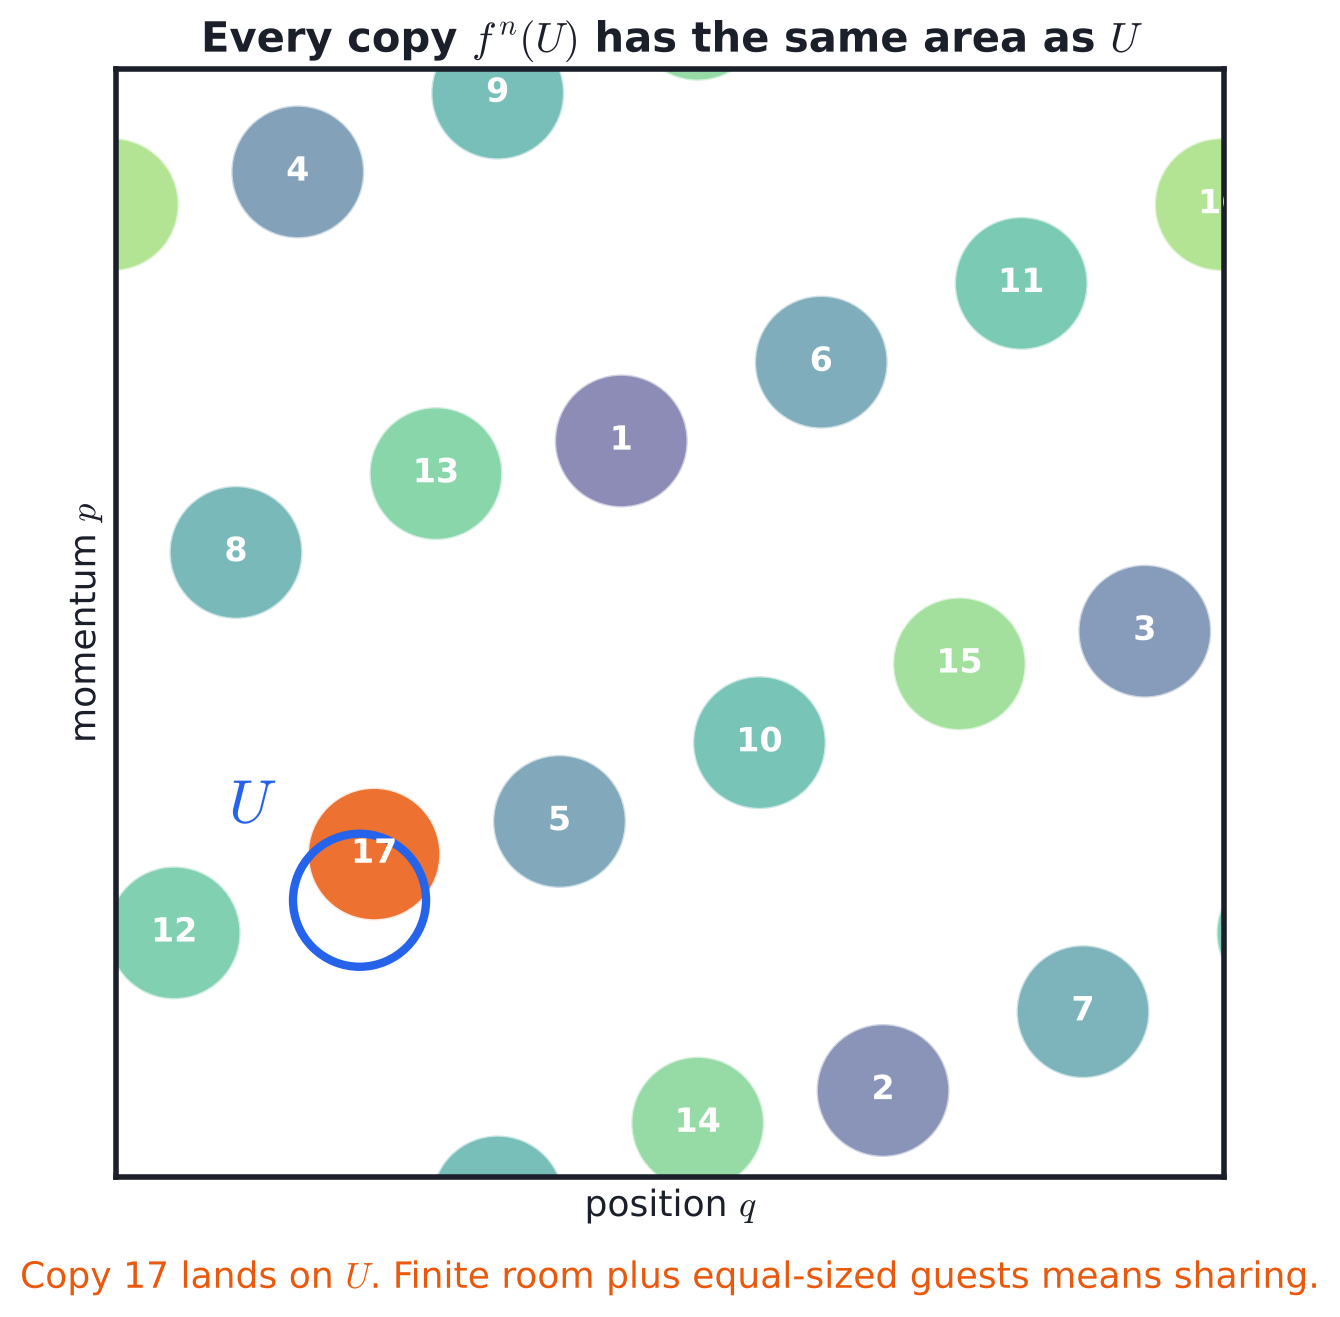
\includegraphics[width=0.52\textwidth]{01_pigeonhole_proof.png}
  \caption{The pigeonhole idea. A disk $U$ is moved by the area-preserving shift $(q,p) \mapsto (q + \sqrt5 - 2,\ p + \sqrt2 - 1) \bmod 1$. Each copy $f^n(U)$ has the same area as $U$ (here about $1.1\%$ of the box). At most about 88 such copies could fit without overlapping. In practice copy 17 already lands on $U$.}
  \label{fig:pigeon}
\end{figure}

%==========================================================================
\section{Why Hamiltonian systems qualify}
\label{sec:liouville}

For the theorem to apply to physics, we need a mechanical system with both properties: no squeezing and finite room.

\subsection{No squeezing: Liouville's theorem}

Take a system with coordinates $q_i$ and momenta $p_i$, $i = 1,\dots,n$, obeying Hamilton's equations
\[
\dot q_i = \frac{\partial H}{\partial p_i}, \qquad \dot p_i = -\frac{\partial H}{\partial q_i}.
\]
These define a velocity field in the $2n$-dimensional phase space. Its divergence is
\[
\nabla\cdot(\dot q,\dot p) \;=\; \sum_{i=1}^{n}\left( \frac{\partial \dot q_i}{\partial q_i} + \frac{\partial \dot p_i}{\partial p_i} \right)
\;=\; \sum_{i=1}^{n}\left( \frac{\partial^2 H}{\partial q_i\,\partial p_i} - \frac{\partial^2 H}{\partial p_i\,\partial q_i} \right) \;=\; 0 ,
\]
since mixed partial derivatives are equal. A region $R(t)$ carried along by the flow changes volume at the rate
\[
\frac{dV}{dt} = \int_{R(t)} \nabla\cdot(\dot q,\dot p)\; d^n q\, d^n p = 0 .
\]
So every volume in phase space is kept fixed. This is Liouville's theorem \cite{goldstein}, and it is exactly the ``measure preserving'' condition.

\subsection{Finite room: bounded energy}

Energy is conserved, so the motion stays on the surface $H = E$. If this surface is bounded (for example, a gas held in a closed box at fixed energy, where walls bound the positions and the energy bounds the momenta), the motion lives in a region of finite volume. Then Poincar\'e's theorem applies.

\subsection{What friction does}

Add a friction force, $\dot p = -\partial H/\partial q - \gamma p$. The divergence becomes $-\gamma$, so $dV/dt = -\gamma V$ and
\[
V(t) = V(0)\, e^{-\gamma t}.
\]
Every region shrinks onto the resting state and nothing comes back. Friction breaks the theorem.

\subsection{Numerical check}

We tested this on a pendulum, $H = p^2/2 - \cos q$. We filled a disk of radius $0.45$ centred at $(q,p) = (0, 1.55)$ with starting points and moved each one with \texttt{scipy}'s DOP853 integrator \cite{hairer} (relative tolerance $10^{-10}$). The area was measured from 20{,}000 points on the boundary with the shoelace formula. Table~\ref{tab:liouville} and Figure~\ref{fig:liouville} show the result.

\begin{table}[H]
  \centering
  \begin{tabular}{lccc}
    \toprule
    case & area at $t=0$ & area at $t=12$ & theory at $t=12$ \\
    \midrule
    no friction & 0.63617 & 0.63616 & 0.63617 \\
    friction, $\gamma = 0.25$ & 0.63617 & 0.03167 & 0.03167 \\
    \bottomrule
  \end{tabular}
  \caption{Area of a blob of pendulum states. The tiny drift without friction comes from the finite number of boundary points once the blob becomes a very thin swirl.}
  \label{tab:liouville}
\end{table}

\begin{figure}[H]
  \centering
  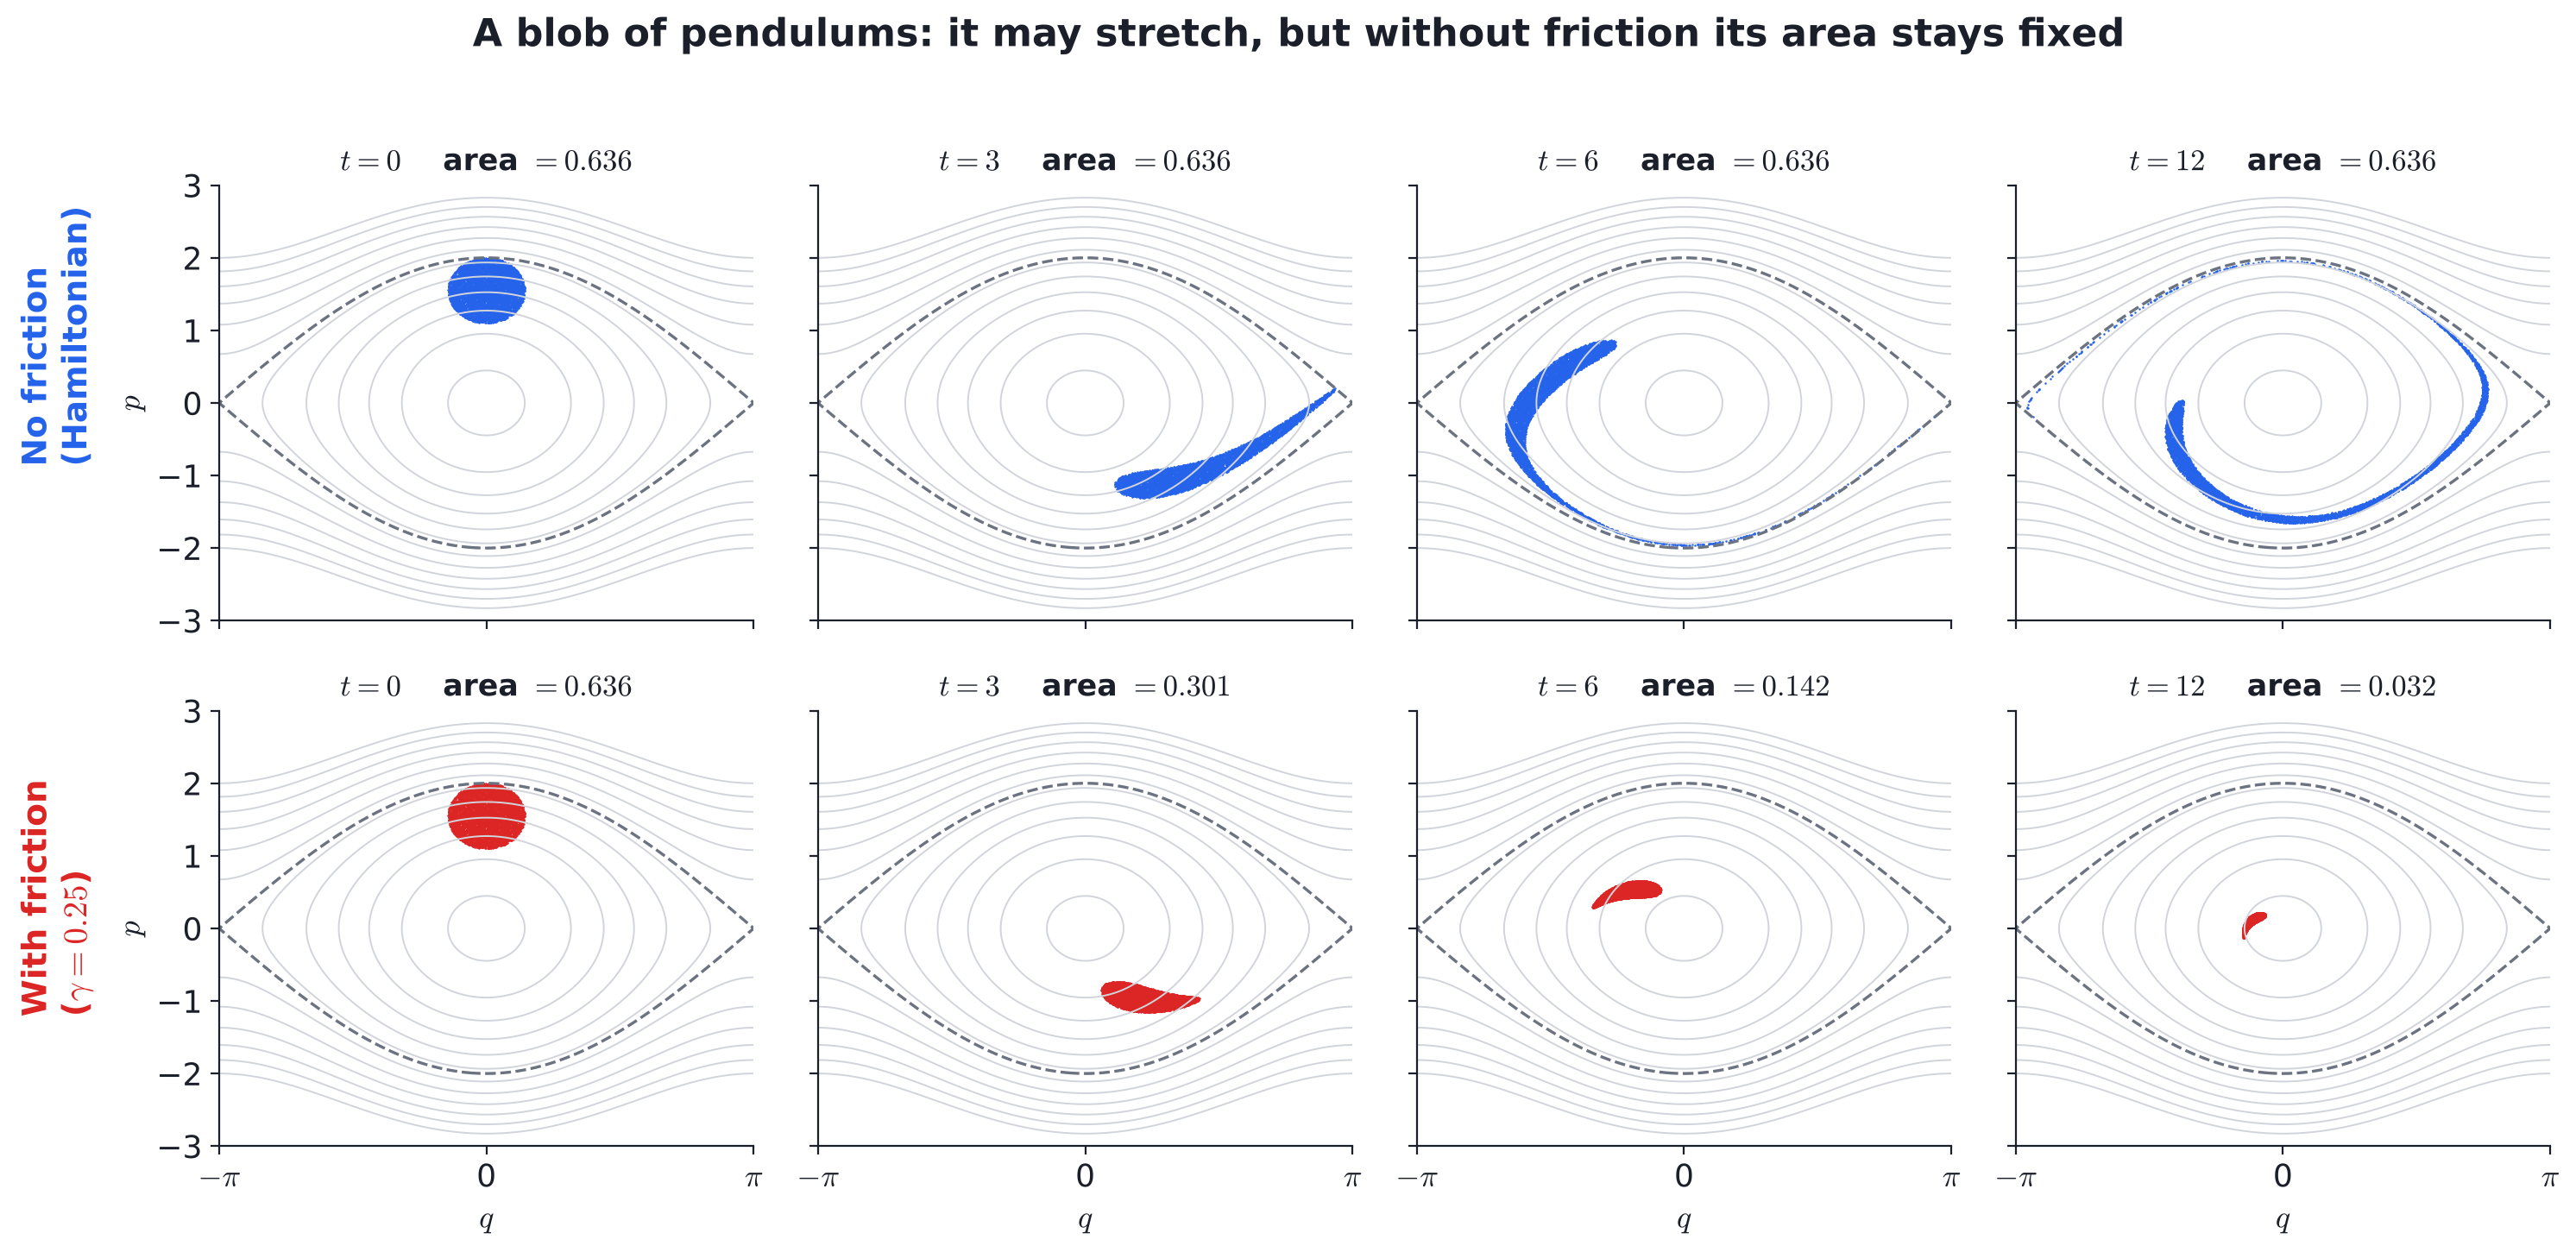
\includegraphics[width=\textwidth]{02_liouville_blobs.png}
  \caption{A blob of pendulum states. Top row: without friction it swirls into a long thin shape but keeps its area. Bottom row: with friction it shrinks to the bottom of the well. Dashed line: the separatrix.}
  \label{fig:liouville}
\end{figure}

%==========================================================================
\section{Two warm-up examples}
\label{sec:examples}

Before the gas, two examples show what recurrence is and what it is not.

\subsection{Two oscillators with an irrational frequency ratio}

Take two uncoupled oscillators, $H = \tfrac12(p_1^2 + \omega_1^2 x_1^2) + \tfrac12(p_2^2 + \omega_2^2 x_2^2)$. Each keeps its own energy, so the state is fixed by two phases $\theta_i = \omega_i t \bmod 2\pi$. The motion is a straight line on a 2-torus, the surface of a doughnut. We chose $\omega_2/\omega_1 = \varphi = (1+\sqrt5)/2$, the golden ratio. Since this is irrational, the line never closes. The motion is never periodic. Even so, by Weyl's theorem \cite{weyl} it passes arbitrarily close to every point of the torus, including its starting point. This is recurrence without repetition (Figure~\ref{fig:torus-osc}).

\textbf{How long until it comes back within $\varepsilon$?} On an $n$-torus a straight-line flow with velocity $\boldsymbol\omega$ spreads evenly, so the fraction of time spent inside a ball $B_\varepsilon$ of volume $V_\varepsilon$ is $V_\varepsilon/(2\pi)^n$. A single pass through the ball takes, on average, the mean chord length divided by the speed. For straight lines crossing a convex body, the mean chord is $V_\varepsilon/\sigma_\varepsilon$, where $\sigma_\varepsilon$ is the cross-section the flow sees ($2\varepsilon$ in two dimensions, $\pi\varepsilon^2$ in three). The mean time between entries is the time per visit divided by the fraction of time inside:
\[
T(\varepsilon) = \frac{V_\varepsilon/(\sigma_\varepsilon |\boldsymbol\omega|)}{V_\varepsilon/(2\pi)^n} = \frac{(2\pi)^n}{|\boldsymbol\omega|\,\sigma_\varepsilon} \;\propto\; \varepsilon^{-(n-1)} .
\]
Every extra oscillator multiplies the wait by another factor of $1/\varepsilon$. Our simulations match this formula to within 1\% for two oscillators and 3\% for three (Figure~\ref{fig:torus-osc}, right). Keep this in mind for the gas: more parts means much longer waits.

\begin{figure}[H]
  \centering
  \begin{subfigure}{0.62\textwidth}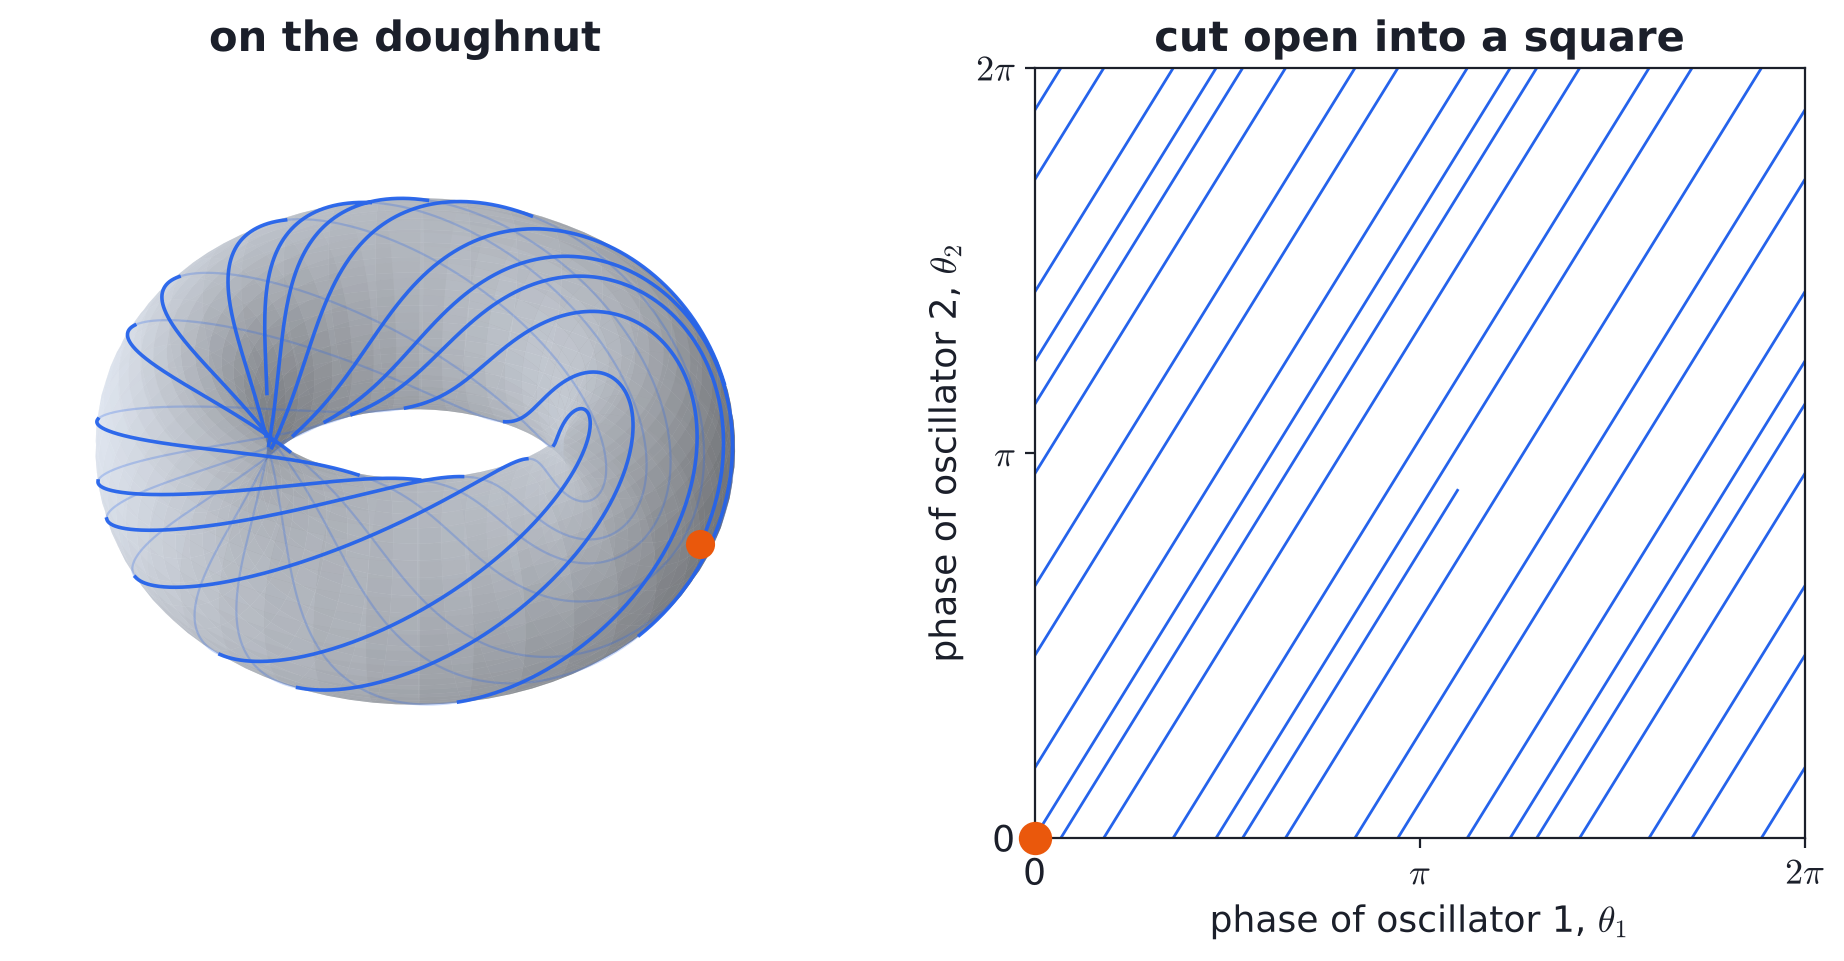
\includegraphics[width=\linewidth]{03_torus.png}\end{subfigure}\hfill
  \begin{subfigure}{0.36\textwidth}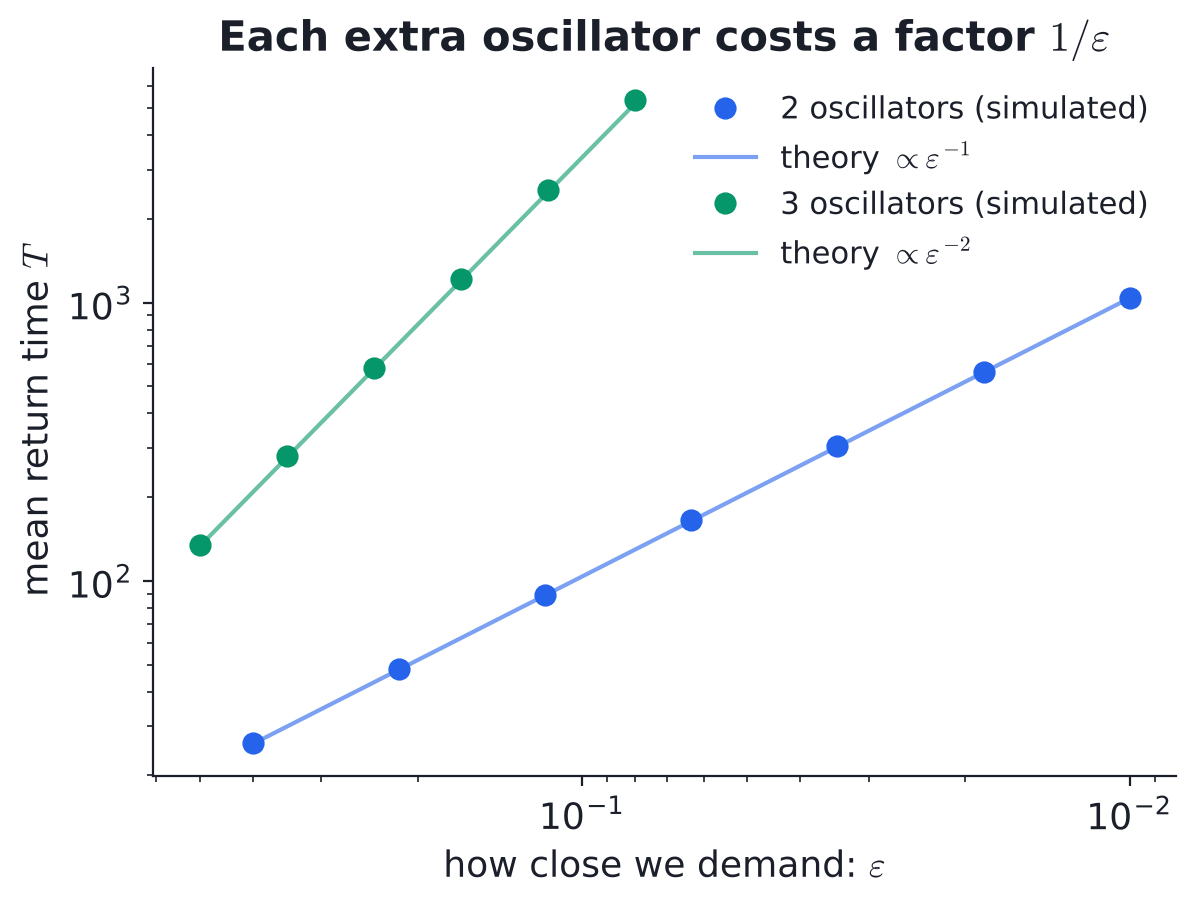
\includegraphics[width=\linewidth]{03_return_scaling.png}\end{subfigure}
  \caption{Left: two oscillators with frequency ratio $\varphi$ wind round a torus without ever closing. Right: mean return time into an $\varepsilon$-ball for two and three oscillators (points) against the formula above (lines).}
  \label{fig:torus-osc}
\end{figure}

\subsection{Arnold's cat map: chaos does not stop recurrence}

The cat map \cite{arnold} acts on the unit square with opposite edges glued:
\[
\begin{pmatrix} x \\ y \end{pmatrix} \mapsto \begin{pmatrix} 2 & 1 \\ 1 & 1 \end{pmatrix}\begin{pmatrix} x \\ y \end{pmatrix} \bmod 1 .
\]
The matrix has determinant 1, so area is preserved. Its eigenvalues are $\lambda_\pm = (3\pm\sqrt5)/2 \approx 2.618$ and $0.382$. Lengths along one direction grow by a factor of 2.618 every step, so nearby points separate exponentially fast, with Lyapunov exponent $\ln 2.618 \approx 0.96$. The map is chaotic.

We applied it to a picture on an $M\times M$ grid of pixels, using the same rule $\bmod\ M$. On the grid the map is a one-to-one shuffle of $M^2$ pixels. Any shuffle of a finite set, repeated enough times, must return to where it began. For $M = 101$ the picture returns exactly after 25 steps (Figure~\ref{fig:cat}). Dyson and Falk showed that the period is never more than $3M$ \cite{dyson}. Chaos changes how fast things get mixed up. It does not stop them coming back. Cats always come home, this one just takes the scenic route.

\begin{figure}[H]
  \centering
  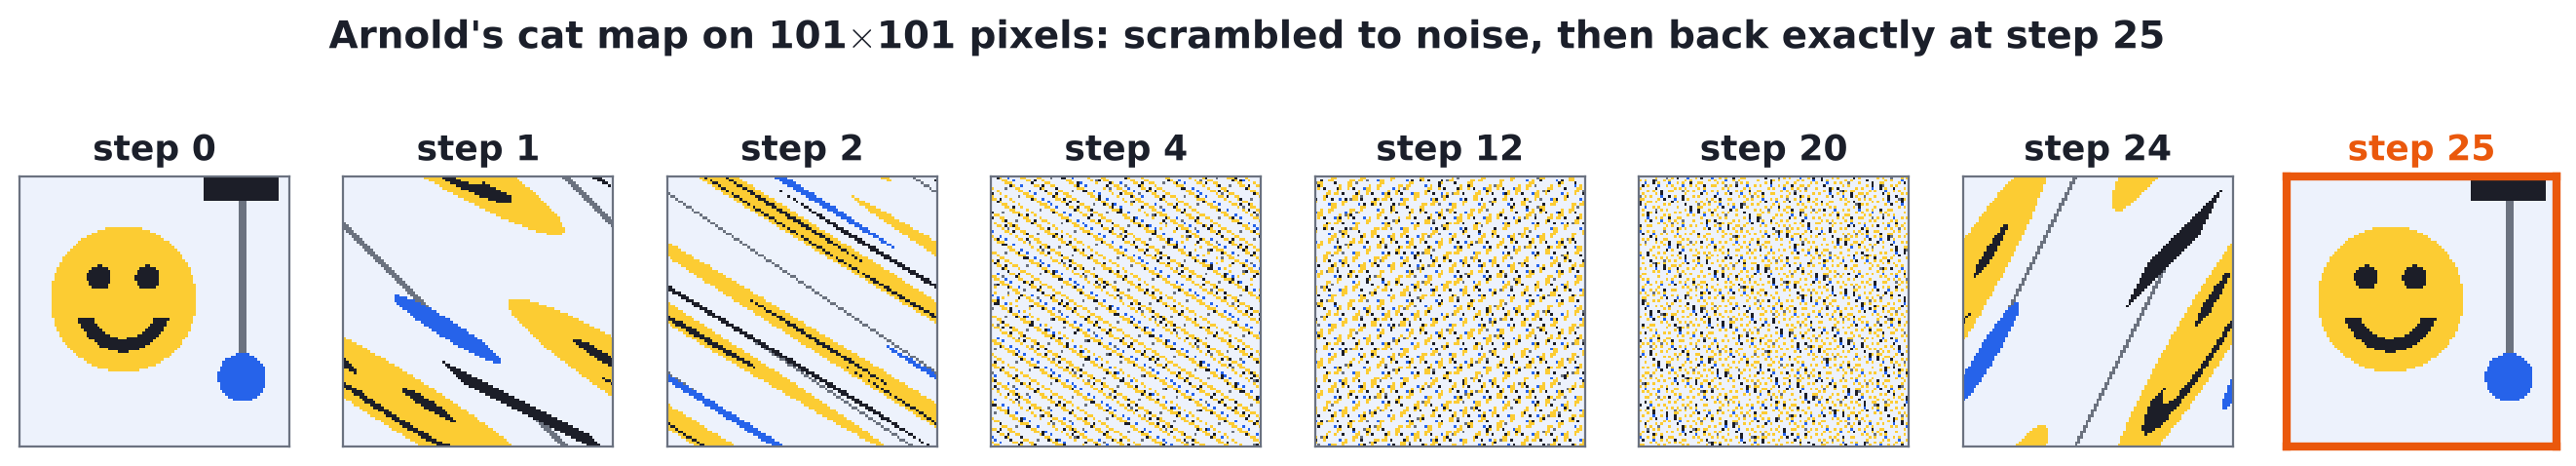
\includegraphics[width=\textwidth]{04_cat_map_strip.png}
  \caption{Arnold's cat map on a $101\times101$ grid. By step 4 the picture looks like noise. At step 25 every pixel is back in place.}
  \label{fig:cat}
\end{figure}

%==========================================================================
\section{Main case: a gas in a box}
\label{sec:gas}

\subsection{Setup}

We place $N$ particles in a square box of side 1. They do not interact with each other and they bounce off the walls elastically. All start in the left half, $x < 1/2$, with random positions and velocities drawn from a normal distribution. We look at the box once per unit of time ($\Delta t = 1$) and ask: at which looks are \emph{all} the particles back in the left half? Since this question only involves the $x$ coordinates, from now on we only track $x$.

\subsection{Each bounce is a circle}
\label{sec:unfold}

A particle bouncing between $x=0$ and $x=1$ with speed $v$ can be ``unfolded''. Let $\theta(t) = (x_0 + v t) \bmod 2$ and
\[
x = \begin{cases} \theta, & 0 \le \theta < 1, \\ 2 - \theta, & 1 \le \theta < 2. \end{cases}
\]
While $\theta < 1$ the particle moves with velocity $+v$, and while $\theta > 1$ it moves with $-v$. The switch at $\theta = 1$ is the bounce off the right wall, and the wrap from $\theta = 2$ back to $0$ is the bounce off the left wall. So the bouncing particle is the same as a point running round a circle of length 2. Half a lap takes it from one wall to the other.

To make the left half of the box a single piece of the circle, we shift the angle by a quarter turn:
\[
\varphi = \left(\theta + \tfrac12\right) \bmod 2 .
\]
The particle is on the left ($x < 1/2$) when $\theta \in [0, \tfrac12) \cup (\tfrac32, 2)$. Adding $\tfrac12$ sends these to $[\tfrac12, 1)$ and $(0, \tfrac12)$, so
\[
x < \tfrac12 \quad\Longleftrightarrow\quad \varphi \in [0, 1) ,
\]
up to the single point $\varphi = 0$, which has zero length. Figure~\ref{fig:torus-idea} (left) shows the circle with its left half in blue.

\subsection{The gas is a point on a torus}

With $N$ particles we have $N$ angles. The state of the gas is the point
\[
\boldsymbol\varphi = (\varphi_1, \dots, \varphi_N) \in \T^N = [0,2)^N ,
\]
where opposite faces of the cube $[0,2)^N$ are glued together. This is the $N$-dimensional torus. Between two looks every angle moves forward by its own velocity, so one look is the map
\[
T(\boldsymbol\varphi) = (\boldsymbol\varphi + \mathbf{v}) \bmod 2, \qquad \mathbf v = (v_1,\dots,v_N) .
\]
The whole gas is a single point jumping in a straight line across the torus. For $N = 2$ the torus is a $2\times2$ square with opposite edges glued, which is a doughnut (Figure~\ref{fig:torus-idea}). For $N = 3$ it is a cube with opposite faces glued. We will not try to draw the ten-dimensional one.

\begin{figure}[H]
  \centering
  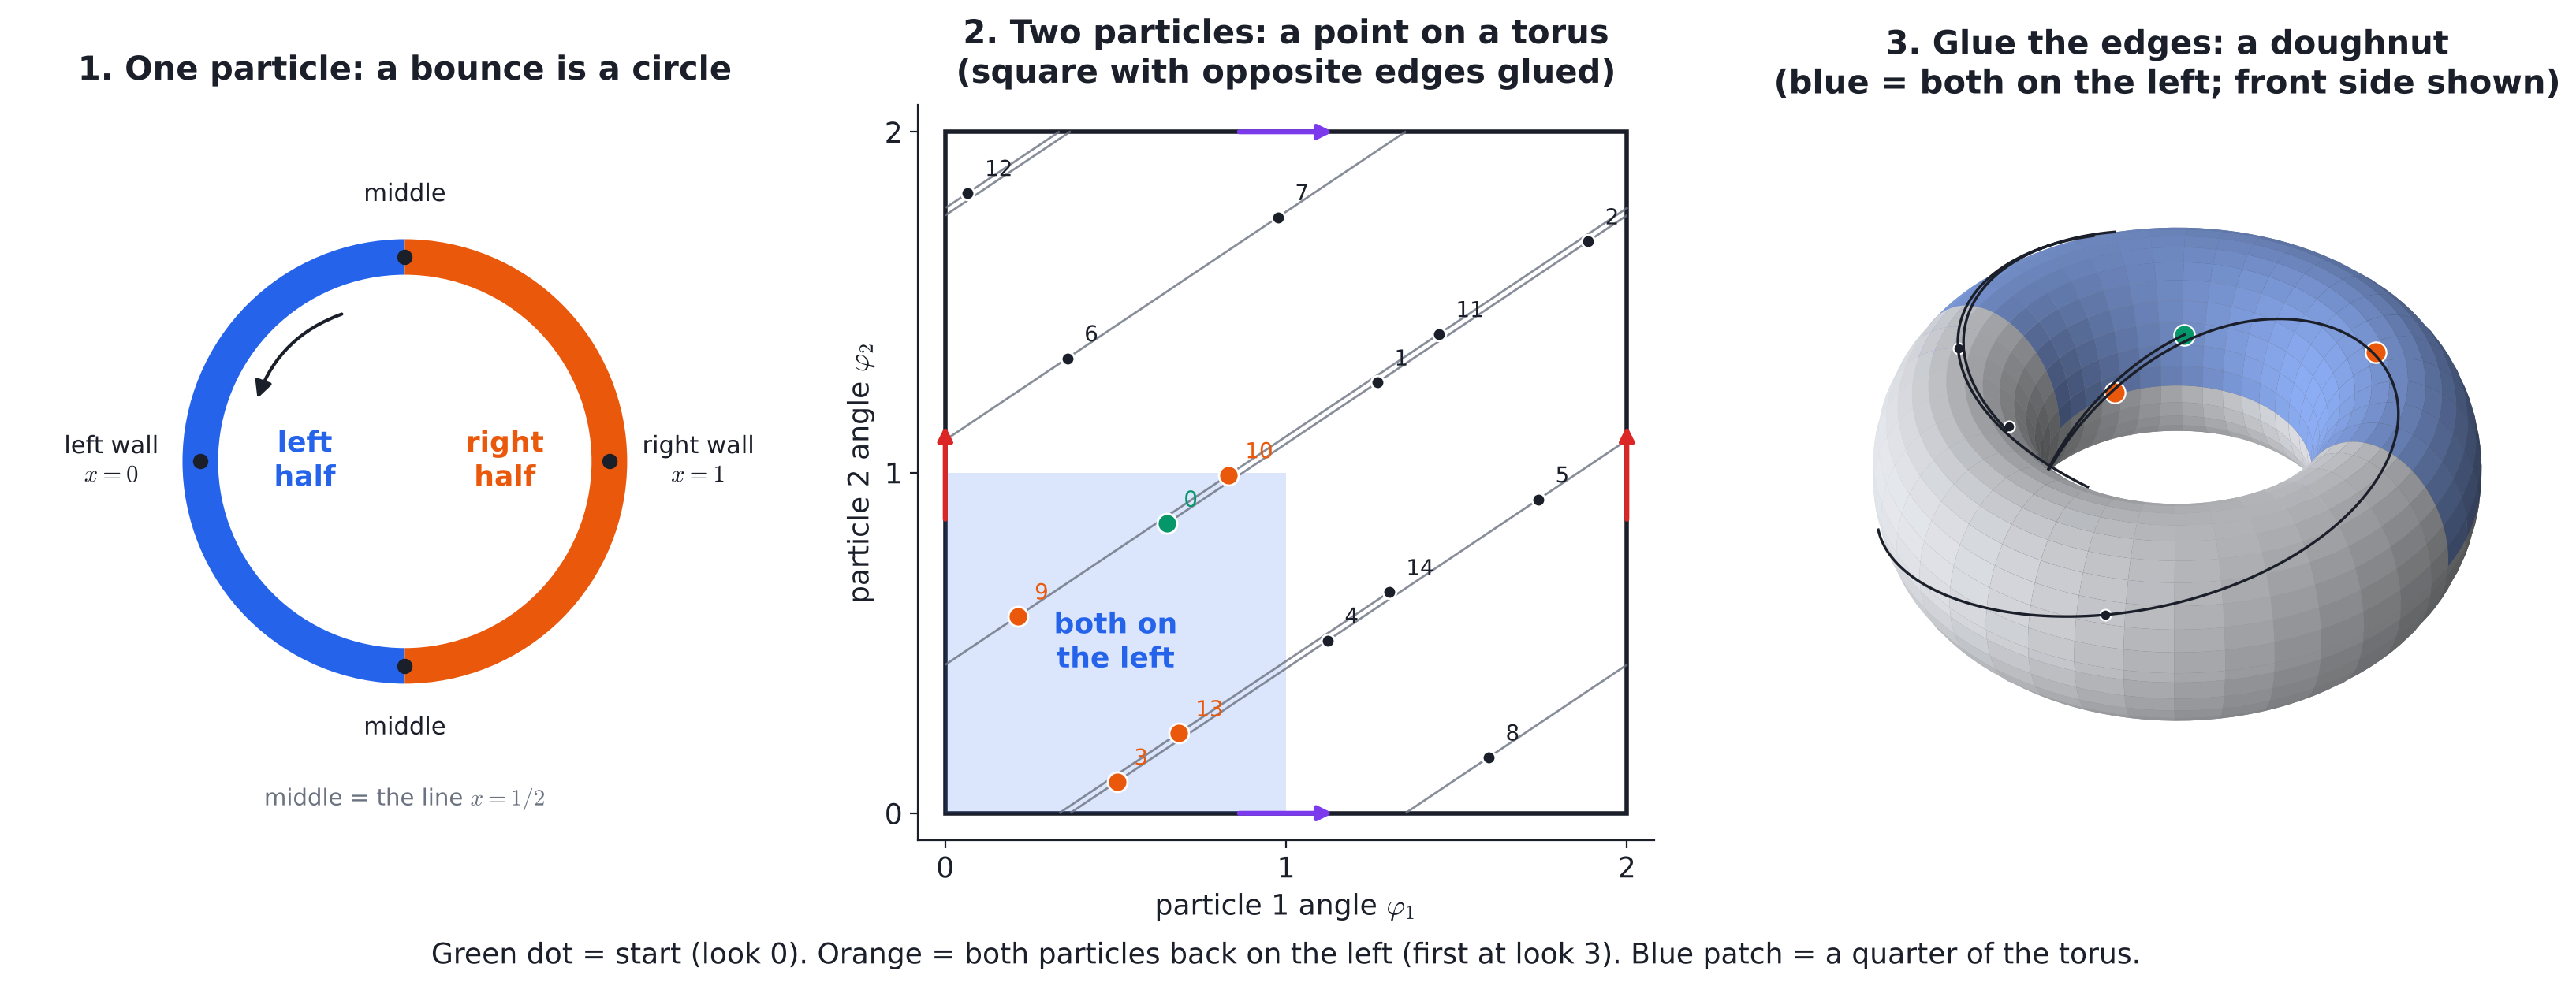
\includegraphics[width=\textwidth]{06_torus_idea.png}
  \caption{From the box to the torus, for $N=2$. Left: one particle's bounce is a circle, with the left half of the box in blue. Middle: two particles are a point in a square with opposite edges glued. Numbered dots are the looks. Orange dots are looks where both particles are on the left. The first return is at look 3. Right: gluing the edges gives a doughnut, with the target region in blue.}
  \label{fig:torus-idea}
\end{figure}

\subsection{Poincar\'e's two conditions}

\textbf{No squeezing.} $T$ is a translation. It moves every set without changing its shape, so $\mu(T^{-1}B) = \mu(B)$ for the usual volume $\mu$.

\textbf{Finite room.} The torus has volume $\mu(\T^N) = 2^N < \infty$.

Both conditions hold, so the gas must keep coming back to ``all on the left''. This is the same argument as Section~\ref{sec:liouville}, but here we can see it directly. Free motion in a box is Hamiltonian, and the translation on the torus is its Liouville flow written in convenient coordinates.

\subsection{Ergodicity: the point fills the torus evenly}

For Kac's lemma we also need the motion to be \emph{ergodic}. Roughly, this means a typical point wanders through the whole space instead of staying in one part. For a translation on a torus there is a clean test due to Weyl \cite{weyl}. The map $\boldsymbol\varphi \mapsto \boldsymbol\varphi + \mathbf v \bmod 2$ is ergodic when the numbers $v_1/2, \dots, v_N/2$ and $1$ are rationally independent. In other words, no relation $k_1 v_1/2 + \dots + k_N v_N/2 = m$ holds with whole numbers $k_i, m$ unless all of them are zero. Velocities drawn from a continuous distribution meet this condition with probability 1.

When the map is ergodic, the looks spread evenly over the torus. The share of looks that land in a region equals that region's share of the volume. Figure~\ref{fig:filling} shows this for $N = 2$. After 400 looks, 97 land in the quarter of the square where both particles are on the left. That is one look in $400/97 \approx 4.1$.

\begin{figure}[H]
  \centering
  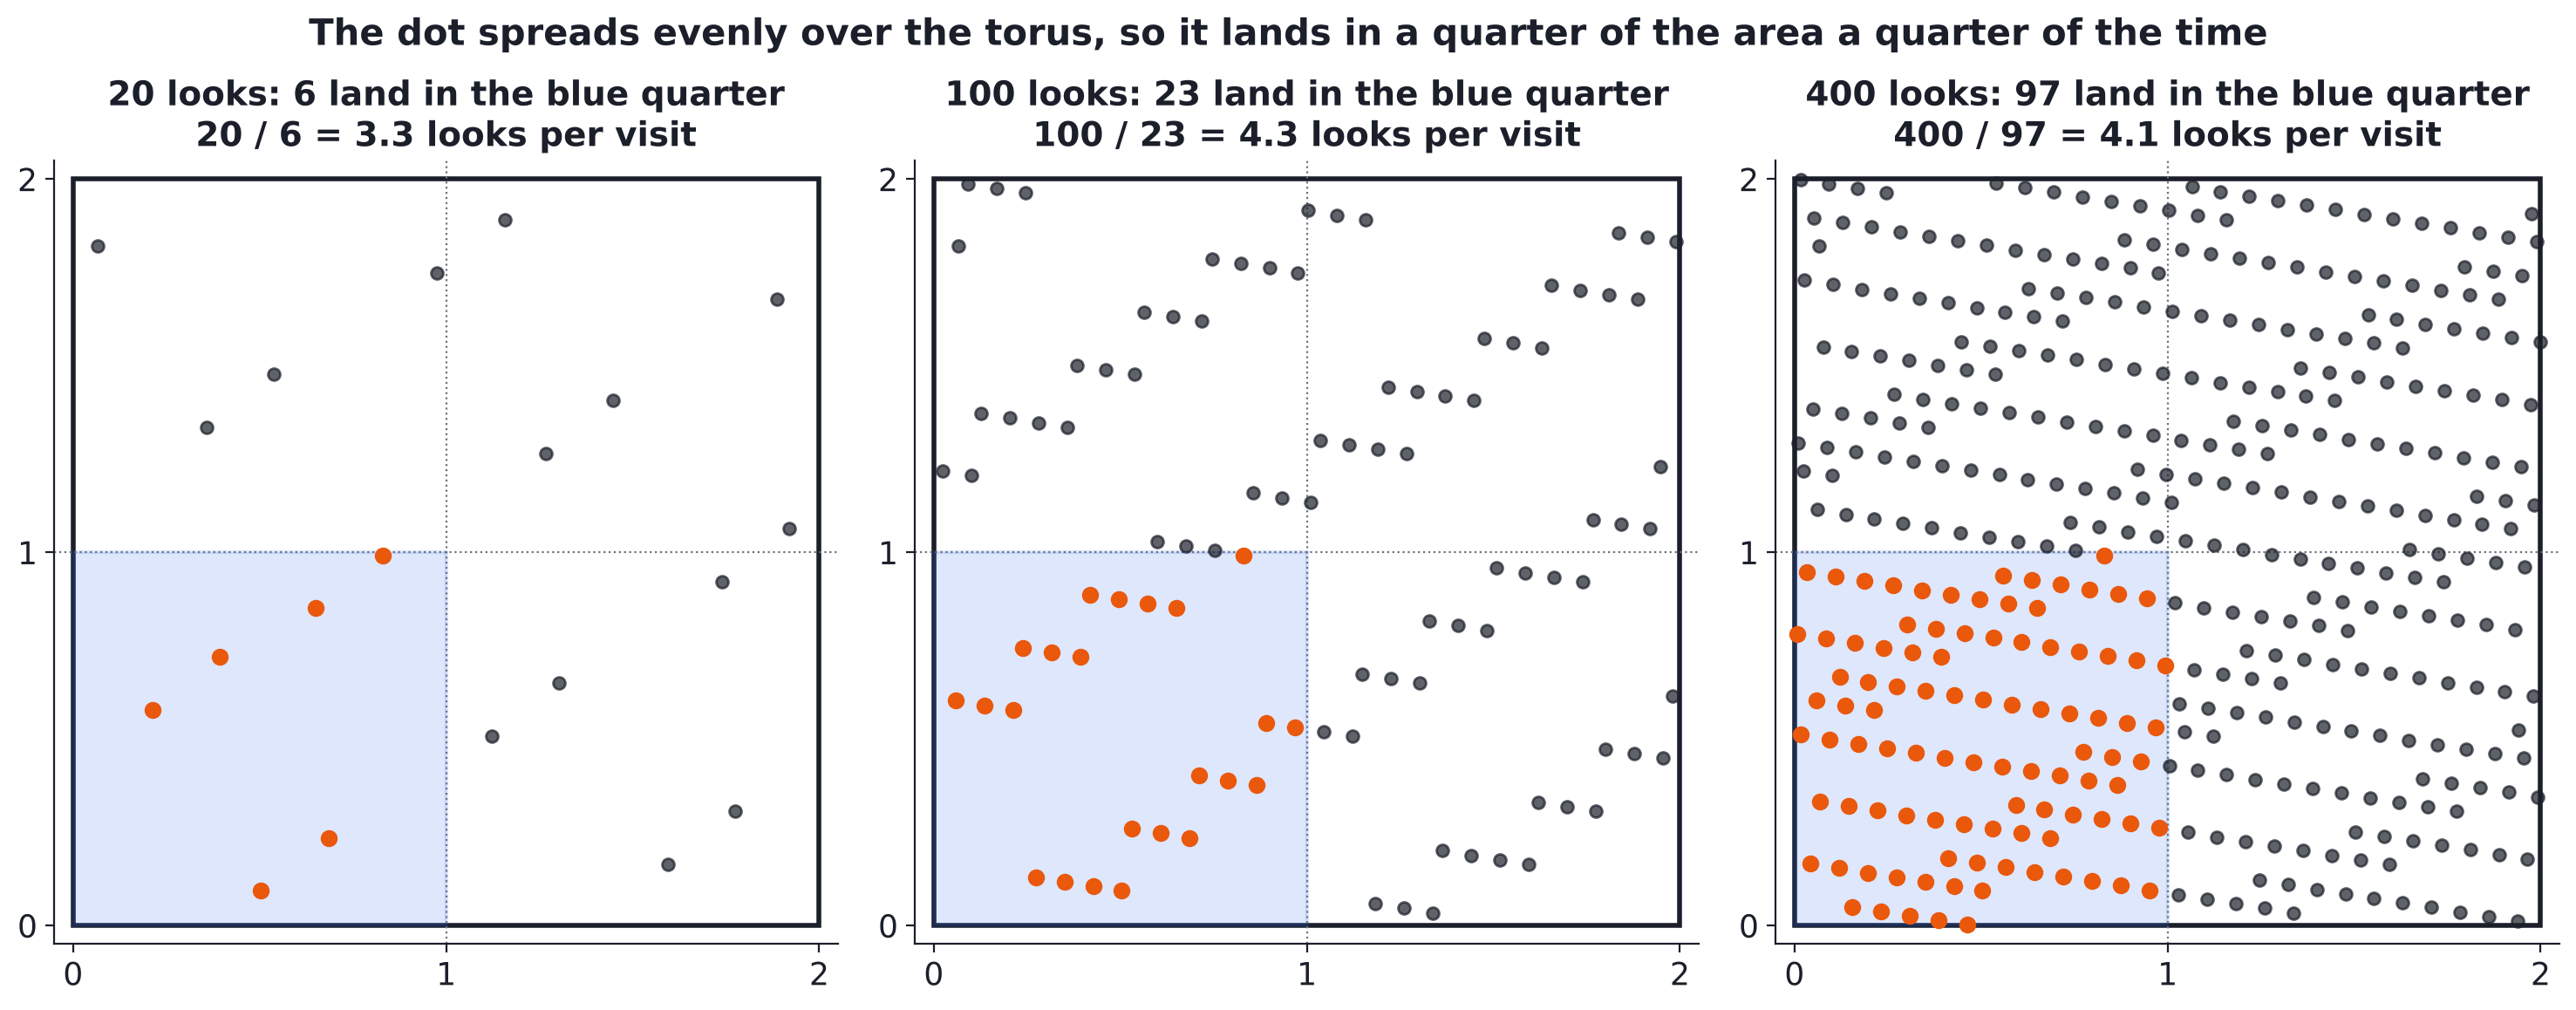
\includegraphics[width=\textwidth]{06_torus_filling.png}
  \caption{The looks of a two-particle gas fill the square torus evenly. The blue quarter is ``both particles on the left''. As the number of looks grows, the share of looks inside it settles at $1/4$.}
  \label{fig:filling}
\end{figure}

\subsection{The size of the target: $2^{-N}$}

``All particles on the left'' means $\varphi_i \in [0,1)$ for every $i$, so the target is the cube
\[
A = [0,1)^N \subset \T^N .
\]
Volume is a product measure. For a set built by choosing one interval for each coordinate, the volume is the product of the lengths. So
\[
\mu(A) = \underbrace{1 \times 1 \times \cdots \times 1}_{N} = 1,
\qquad
\frac{\mu(A)}{\mu(\T^N)} = \frac{1}{2^N} = 2^{-N} .
\]
This product rule works because the target is a ``box'' set. Each particle's condition only involves its own angle, which is the same as saying the particles move independently. It would not work for a mixed condition such as ``exactly half of the particles on the left''.

Geometrically, each new particle adds one more direction to the torus, and the target keeps only the half of that direction where the new particle is on the left. So the target halves every time (Figure~\ref{fig:steps}).

\begin{figure}[H]
  \centering
  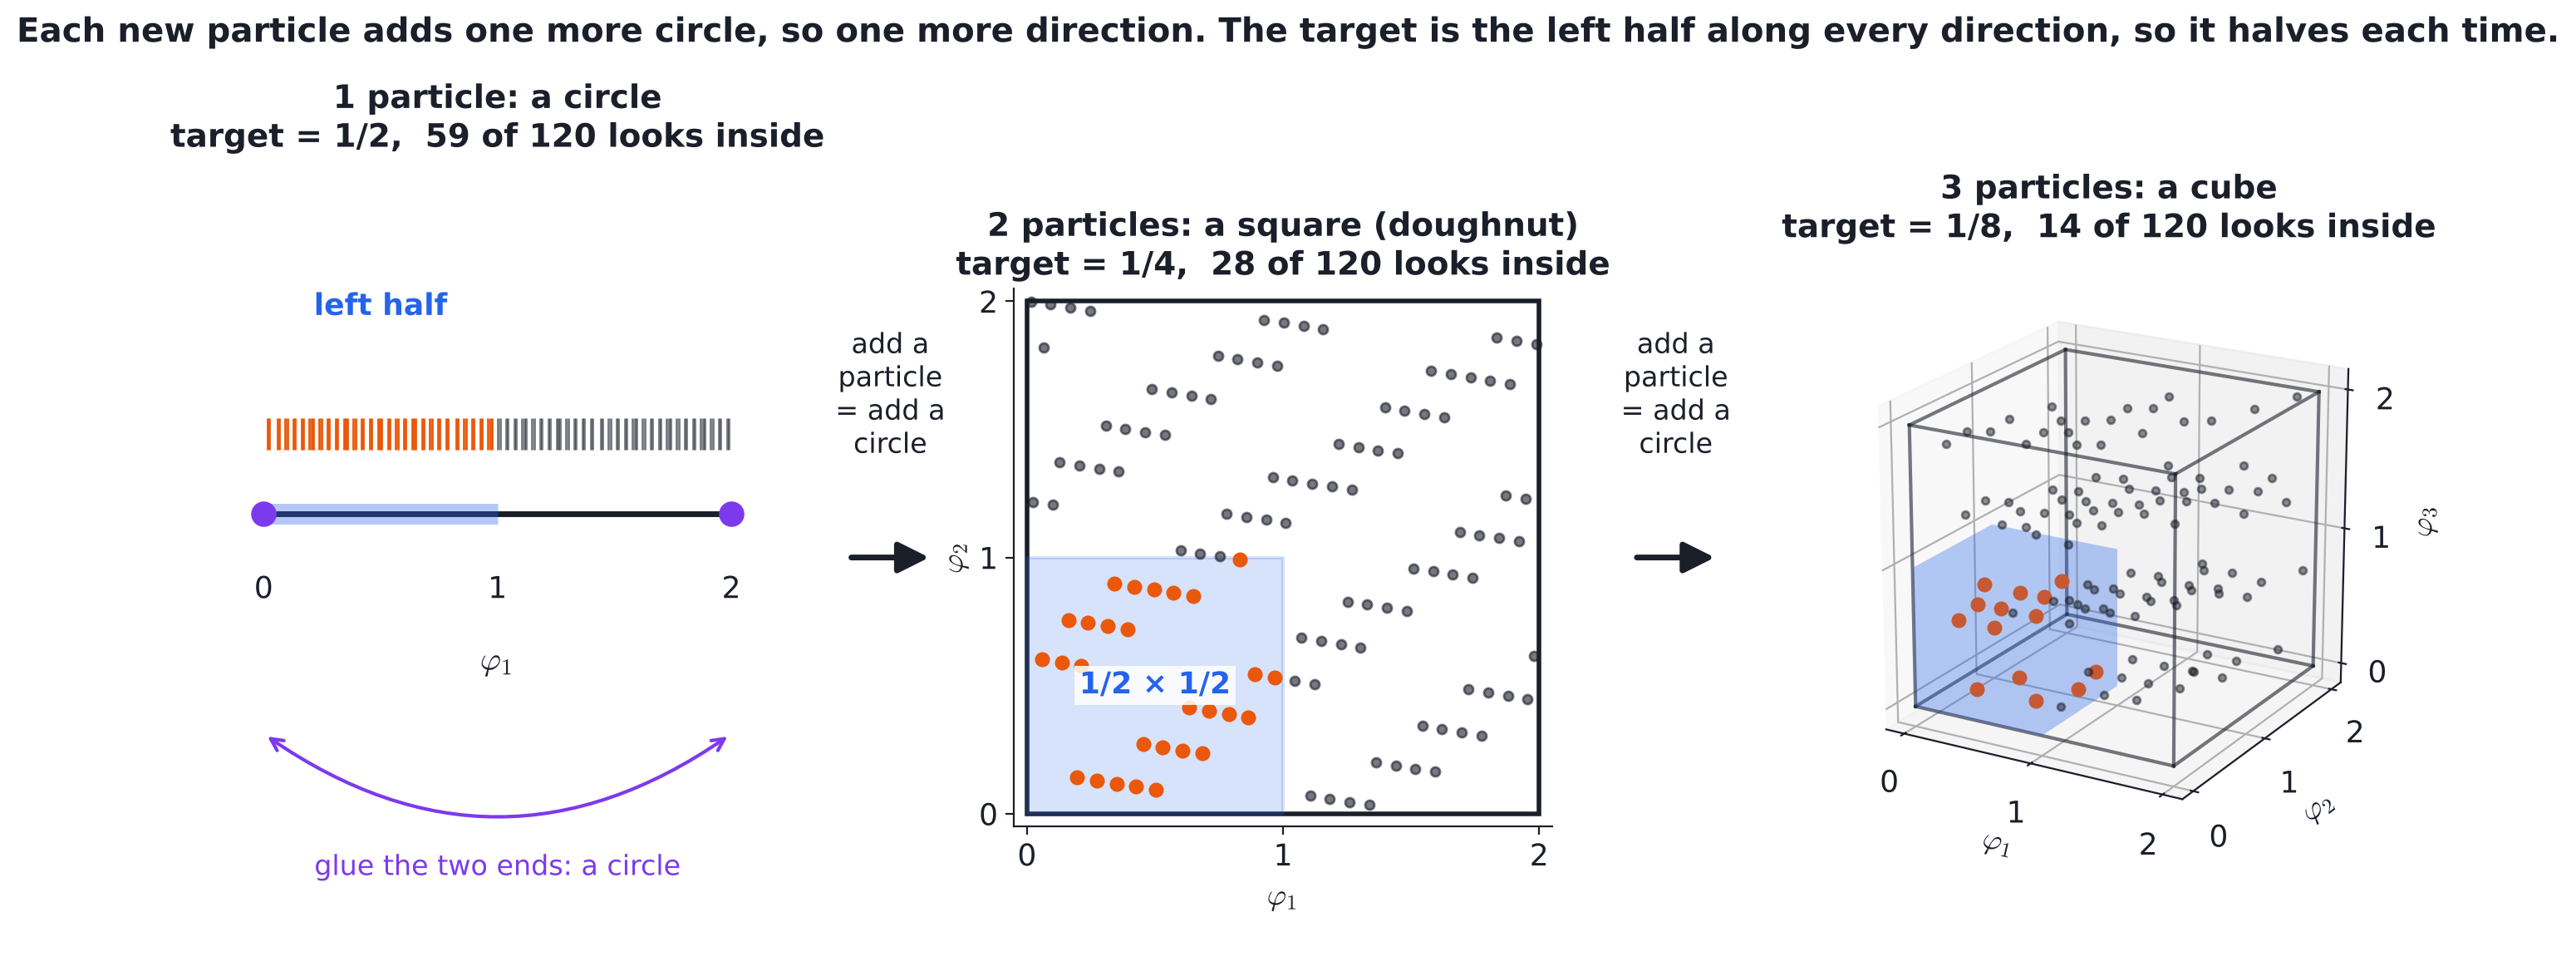
\includegraphics[width=\textwidth]{06_torus_steps.png}
  \caption{Going up one dimension at a time with the same 120 looks. One particle: a circle, target $1/2$, 59 looks inside. Two particles: a square, target $1/4$, 28 inside. Three particles: a cube, target $1/8$, 14 inside.}
  \label{fig:steps}
\end{figure}

\subsection{How long to wait: Kac's lemma}
\label{sec:kac}

Poincar\'e tells us the gas comes back. Kac's lemma tells us how often \cite{kac}.

\begin{lemma}[Kac, 1947]
Let $T$ be measure preserving and ergodic on $\Omega$ with $\mu(\Omega) < \infty$, and let $\mu(A) > 0$. Then the mean return time to $A$, averaged over starting points in $A$, is
\[
\avg{T_A} = \frac{\mu(\Omega)}{\mu(A)} .
\]
\end{lemma}

\textit{Proof sketch.} Normalise so that $\mu(\Omega) = 1$. Split $A$ into pieces $A_n$, where $A_n$ holds the points whose first return to $A$ happens at step $n$. A point of $A_n$ visits the sets $A_n, TA_n, \dots, T^{n-1}A_n$ before it gets back. These sets, over all $n$ and all $0 \le k < n$, do not overlap, and by ergodicity they fill $\Omega$ up to zero volume. Each $T^k A_n$ has volume $\mu(A_n)$, so
\[
\sum_{n \ge 1} n\, \mu(A_n) = \mu(\Omega) = 1 .
\]
The mean return time is $\sum_n n\,\mu(A_n) / \mu(A) = 1/\mu(A)$. \qed

There is also a quick counting argument. In a long run of $L$ looks, the point lands in $A$ about $\mu(A)L/\mu(\Omega)$ times. The gaps between these visits fill the run, so the mean gap is about $L$ divided by the number of visits, which is $\mu(\Omega)/\mu(A)$.

For the gas, $\mu(\T^N)/\mu(A) = 2^N$, so
\[
\boxed{\;\avg{T} = 2^N \text{ looks}\;}
\]
One particle comes back to the left every 2 looks on average, two particles every 4, three every 8, and each extra particle doubles the wait (Figure~\ref{fig:dims}).

\begin{figure}[H]
  \centering
  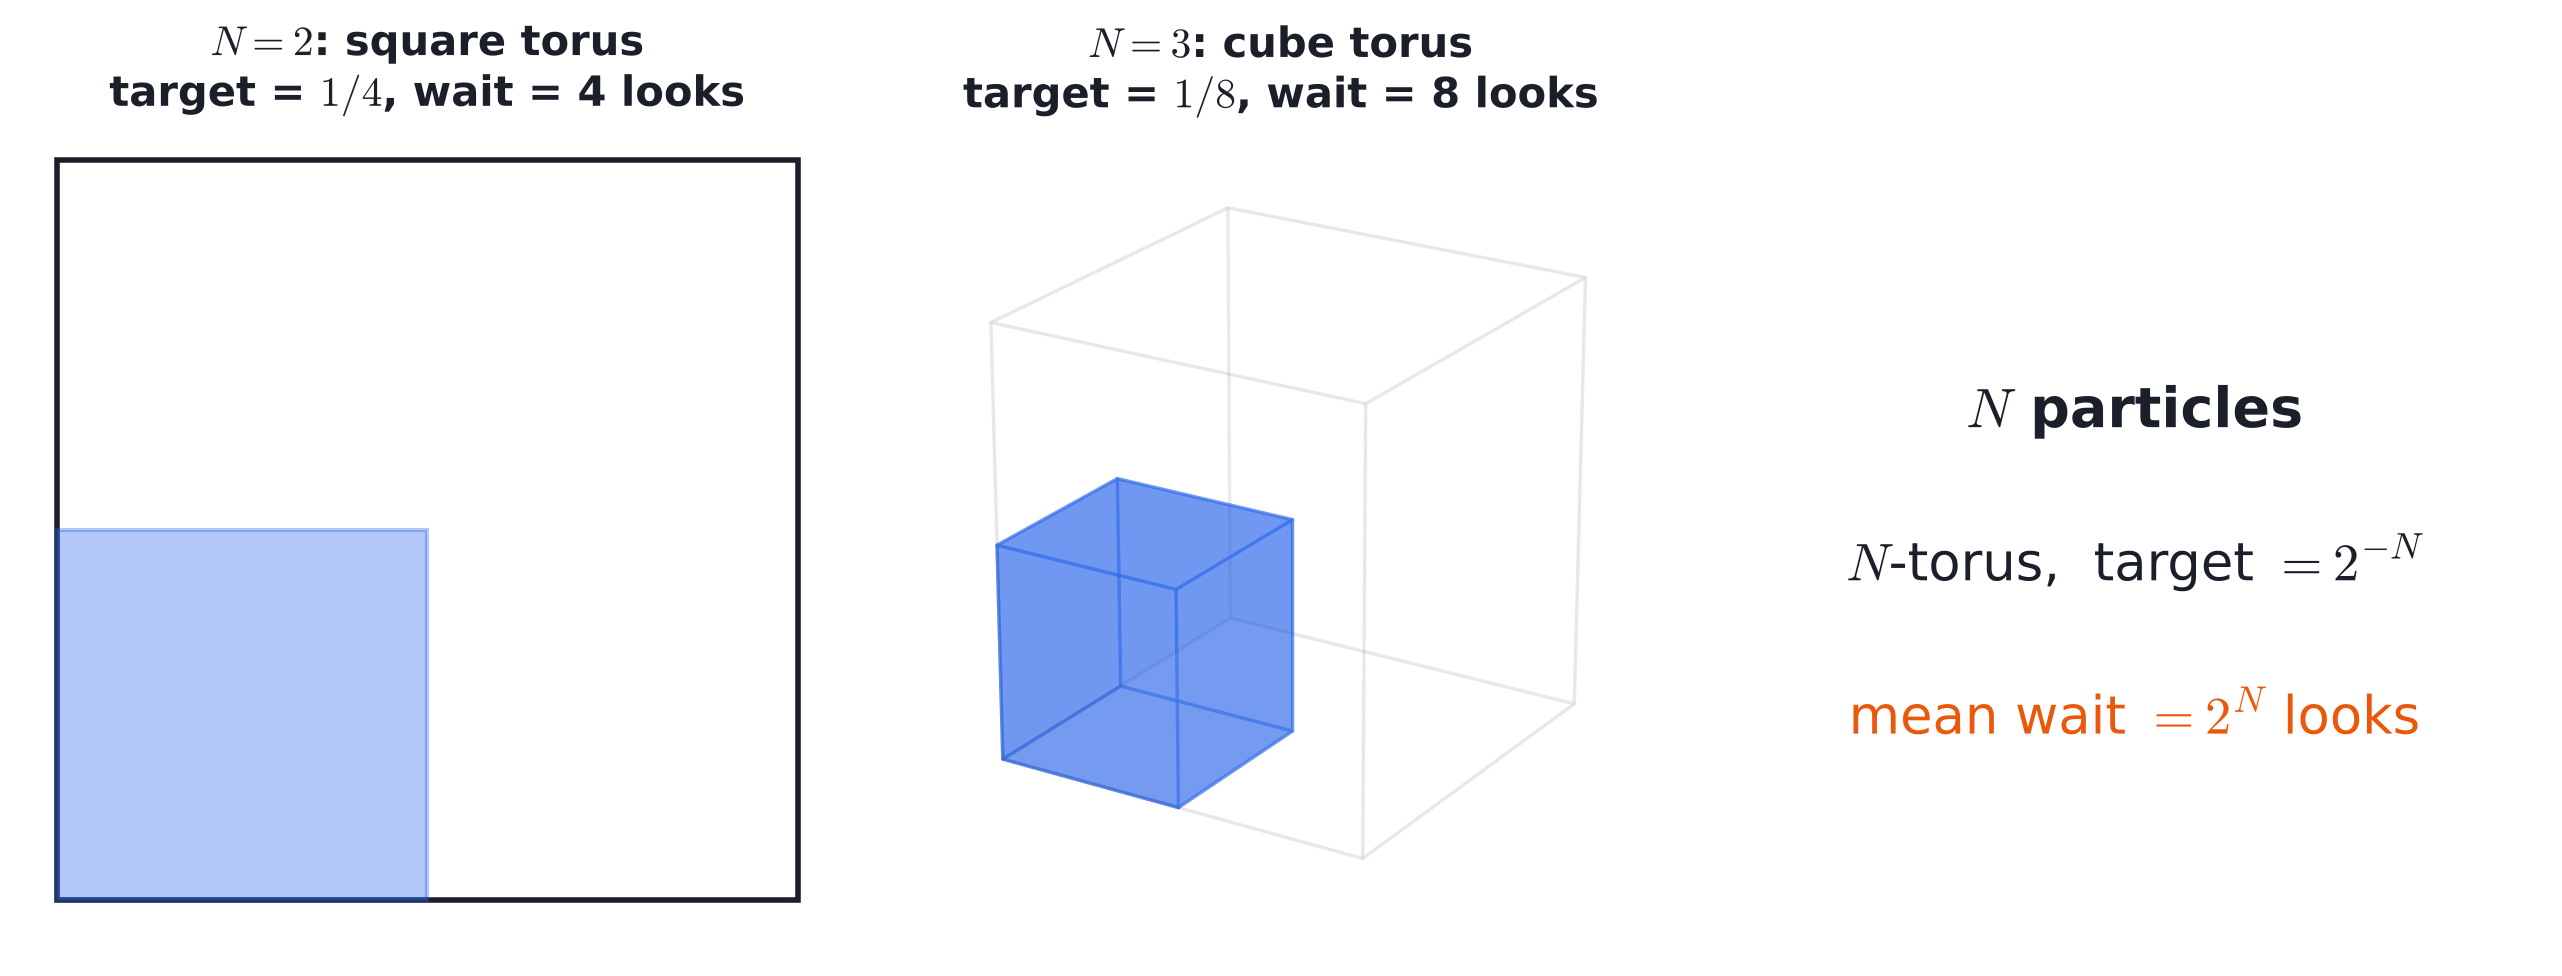
\includegraphics[width=0.85\textwidth]{06_torus_dimensions.png}
  \caption{The target is half of each direction, so it is $1/4$ of the square torus, $1/8$ of the cube torus, and $2^{-N}$ of the $N$-torus. The mean wait is the inverse.}
  \label{fig:dims}
\end{figure}

\subsection{Numerical method}

Because the particles are free, we never need to integrate equations of motion. The position at look $k$ comes straight from the unfolding of Section~\ref{sec:unfold}, $x_i(k) = \mathrm{bounce}(x_i(0) + v_i k)$. So there is no build-up of integration error, however long the run. For each $N$ from 1 to 14 we:
\begin{enumerate}
  \item drew starting positions uniformly in $[0, \tfrac12)$ and velocities from a standard normal distribution (random seed 7),
  \item computed all positions at looks $k = 1, 2, \dots, K$ with $K = \min(4000 \cdot 2^N,\ 6\times10^7)$, in chunks of $10^6$ looks to save memory,
  \item recorded every look at which all $x_i < 1/2$, and took the gaps between consecutive such looks,
  \item reported the mean gap and its standard error $s/\sqrt{n}$, where $s$ is the sample standard deviation of the gaps and $n$ the number of gaps.
\end{enumerate}
This gives about 4000 returns for every $N$ (3557 for $N = 14$, where the run length hit the cap). The standard error treats the gaps as independent, which is a slight simplification since consecutive gaps of a translation are correlated. The full code is in Appendix~\ref{app:code}.

\subsection{Results}

Figure~\ref{fig:snapshots} shows ten particles spreading out and then, at look 89, all being on the left again. That single wait is much shorter than the Kac average of $2^{10} = 1024$ looks. Individual waits vary a lot. Only the average is fixed.

\begin{figure}[H]
  \centering
  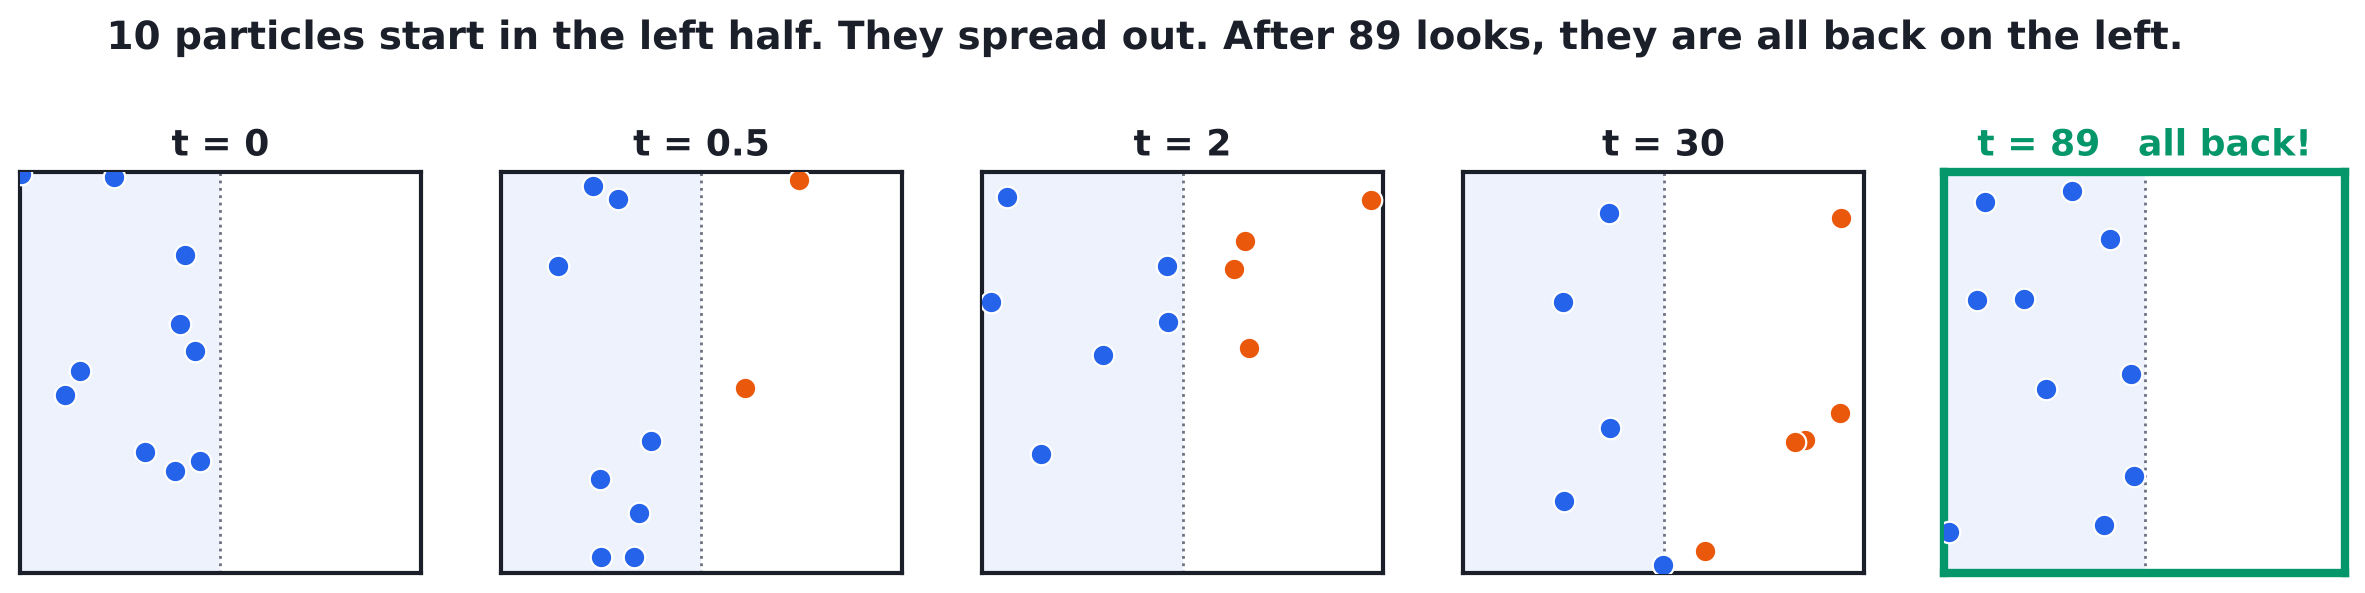
\includegraphics[width=\textwidth]{05_gas_snapshots.png}
  \caption{Ten particles start in the left half (blue). They spread out. At look 89 they are all on the left again.}
  \label{fig:snapshots}
\end{figure}

Figure~\ref{fig:leftfrac} follows the fraction of particles on the left over 6000 looks. With $N = 10$ it reaches 1 five times. With $N = 40$ it never does, which is no surprise, since the expected wait is about $2^{40} \approx 10^{12}$ looks.

\begin{figure}[H]
  \centering
  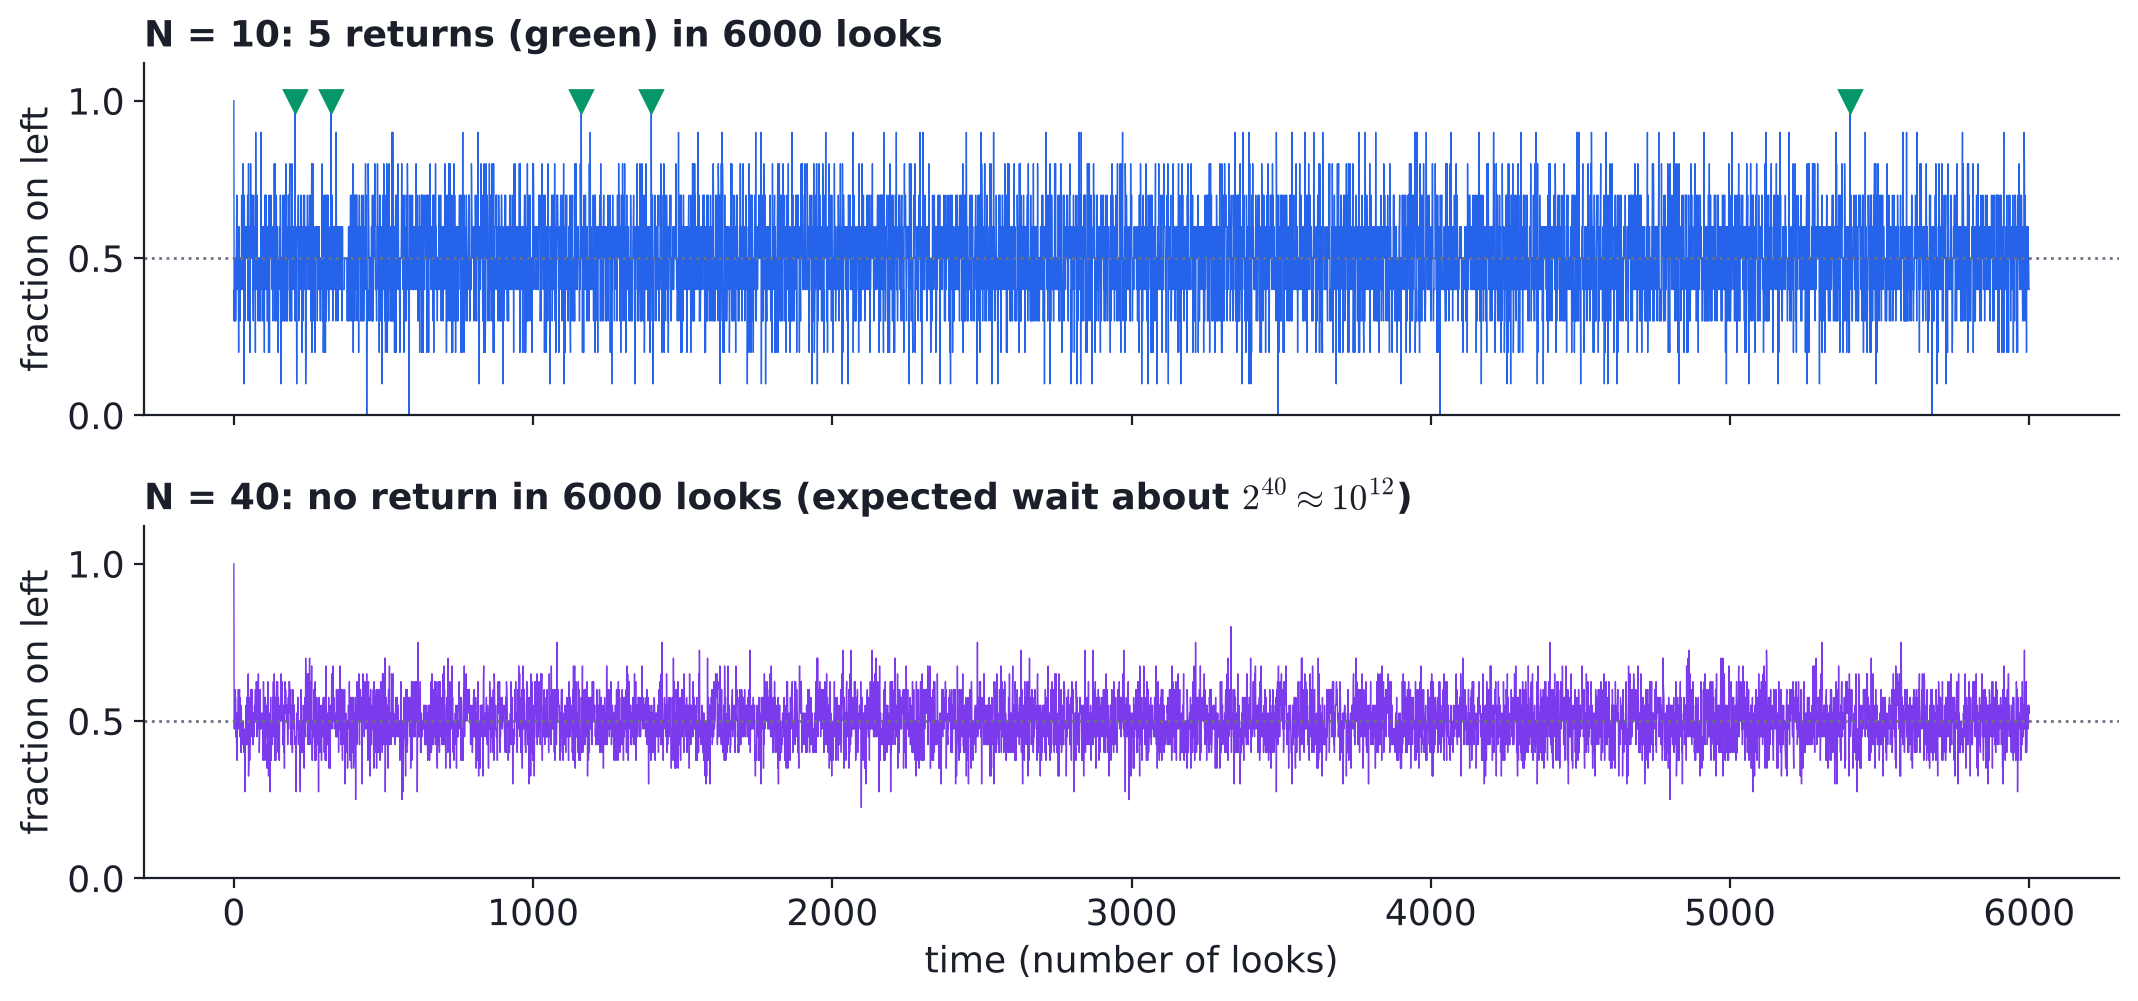
\includegraphics[width=0.9\textwidth]{05_left_fraction.png}
  \caption{Fraction of particles in the left half over 6000 looks. Green markers: all particles on the left. The band for $N=40$ is also much narrower than for $N=10$ (Section~\ref{sec:fluct}).}
  \label{fig:leftfrac}
\end{figure}

Table~\ref{tab:kac} and Figure~\ref{fig:kac} compare the measured mean wait with Kac's prediction for $N = 1$ to $14$. Over this range the wait grows by a factor of about 8000. The measured values agree with $2^N$ to within two standard errors at every $N$. The largest deviation is $1.77$ standard errors, at $N = 5$. With 14 points we expect about two to sit more than $1.5$ standard errors away by chance. We see four. That is a little high, and it fits the slight underestimate of the error bars noted above.

\begin{table}[H]
  \centering
  \begin{tabular}{rrrrr}
    \toprule
    $N$ & returns counted & measured $\avg{T}$ & Kac $2^N$ & deviation (std.\ errors) \\
    \midrule
     1 & 4000 &      2.00 $\pm$ 0.01 &     2 & $-0.04$ \\
     2 & 4000 &      4.00 $\pm$ 0.05 &     4 & $-0.01$ \\
     3 & 4014 &      7.97 $\pm$ 0.25 &     8 & $-0.11$ \\
     4 & 3998 &     16.00 $\pm$ 0.17 &    16 & $+0.02$ \\
     5 & 3917 &     32.7 $\pm$ 0.4   &    32 & $+1.77$ \\
     6 & 4009 &     63.8 $\pm$ 0.9   &    64 & $-0.21$ \\
     7 & 4074 &    125.6 $\pm$ 1.5   &   128 & $-1.53$ \\
     8 & 3956 &    258.7 $\pm$ 4.0   &   256 & $+0.69$ \\
     9 & 3984 &    513.7 $\pm$ 7.1   &   512 & $+0.24$ \\
    10 & 3904 &   1049 $\pm$ 16      &  1024 & $+1.57$ \\
    11 & 4031 &   2031 $\pm$ 31      &  2048 & $-0.54$ \\
    12 & 4023 &   4070 $\pm$ 76      &  4096 & $-0.34$ \\
    13 & 4020 &   8148 $\pm$ 122     &  8192 & $-0.36$ \\
    14 & 3557 &  16866 $\pm$ 292     & 16384 & $+1.65$ \\
    \bottomrule
  \end{tabular}
  \caption{Mean number of looks between returns to ``all particles on the left''. Raw numbers are in \texttt{figures/05\_results.csv}.}
  \label{tab:kac}
\end{table}

\begin{figure}[H]
  \centering
  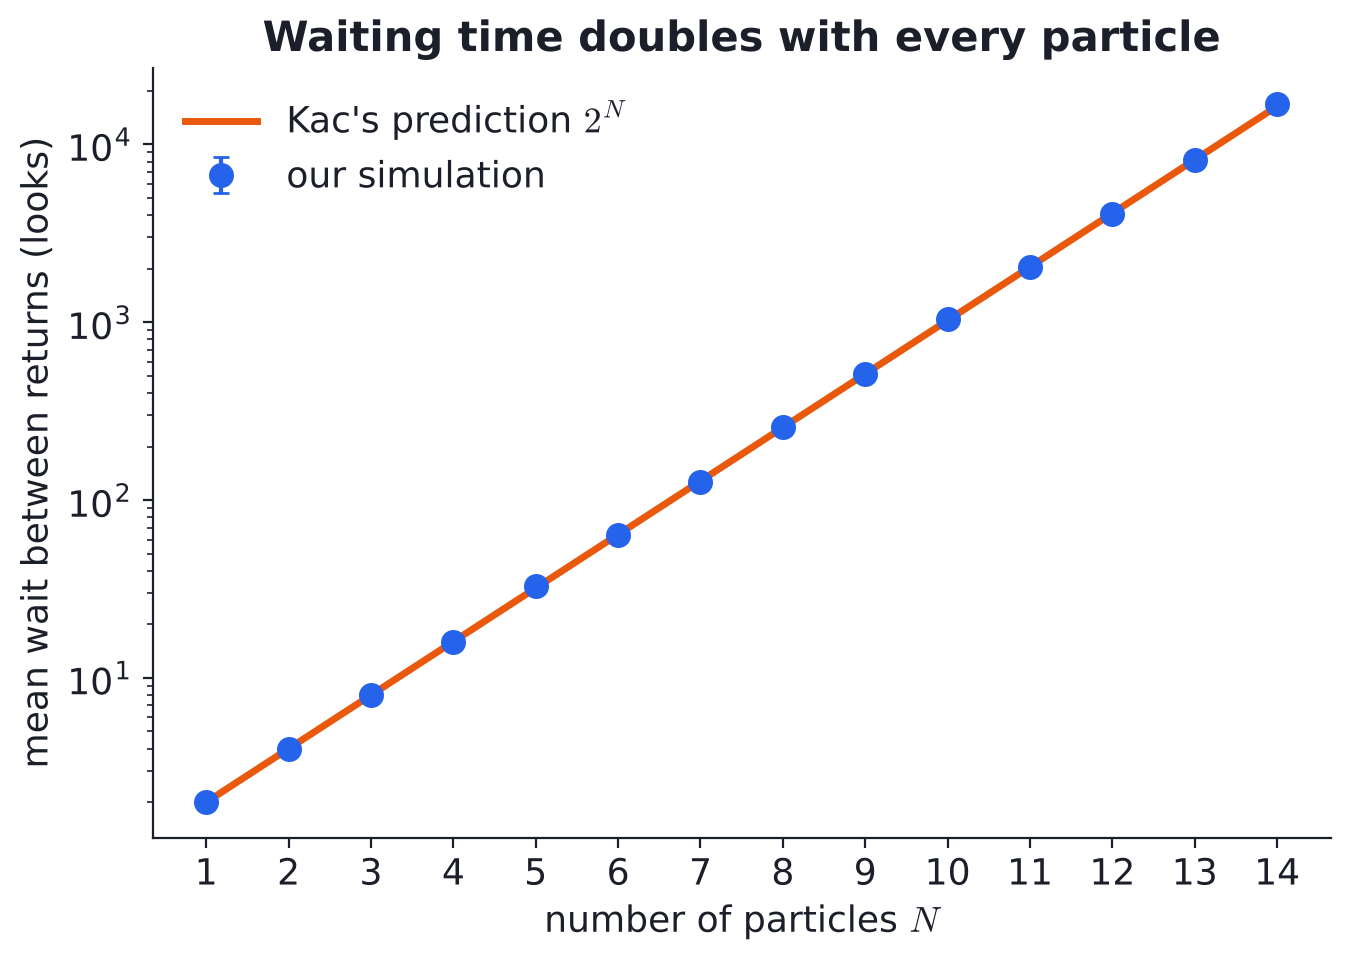
\includegraphics[width=0.62\textwidth]{05_kac_scaling.png}
  \caption{Measured mean wait (points with error bars) against Kac's prediction $2^N$ (line), on a log scale. The wait doubles with every particle.}
  \label{fig:kac}
\end{figure}

%==========================================================================
\section{Interpretation}
\label{sec:interp}

\subsection{How long is ``eventually''?}

Kac's formula lets us go far beyond what we can simulate. Table~\ref{tab:times} assumes one look every millisecond.

\begin{table}[htbp]
  \centering
  \begin{tabular}{rll}
    \toprule
    $N$ & mean wait $2^N$ looks & at one look per millisecond \\
    \midrule
    10 & $1.0\times10^{3}$ & about 1 second \\
    20 & $1.0\times10^{6}$ & about 17 minutes \\
    30 & $1.1\times10^{9}$ & about 12 days \\
    40 & $1.1\times10^{12}$ & about 35 years \\
    60 & $1.2\times10^{18}$ & about 37 million years \\
    100 & $1.3\times10^{30}$ & about $4\times10^{19}$ years \\
    \bottomrule
  \end{tabular}
  \caption{Mean wait for all $N$ particles to be in the left half at once.}
  \label{tab:times}
\end{table}

The age of the universe is about $1.4\times10^{10}$ years, so a hundred particles already need about three billion universe lifetimes. The air in a room holds roughly $10^{27}$ molecules. Its wait, $2^{10^{27}}$ looks, is a number with about $3\times10^{26}$ digits. Nobody in the room needs to worry about breathing.

\subsection{Why a big gas looks evenly spread}
\label{sec:fluct}

Recurrence is not only rare for a large gas. The gas also rarely strays far from half and half. Because the looks fill the torus evenly and the volume is a product measure, each particle is on the left in an independent half of the looks. The number on the left is then binomial with mean $N/2$, and the fraction on the left has mean $1/2$ and standard deviation
\[
\sigma = \frac{1}{2\sqrt N} .
\]
From the runs in Figure~\ref{fig:leftfrac} we measured $\sigma = 0.158$ for $N = 10$ and $0.079$ for $N = 40$, matching the formula (0.158 and 0.079). For $N = 10^{27}$ the spread is about $2\times10^{-14}$. A real gas always looks evenly spread, even though it is guaranteed to come back to every unusual state given enough time.

\subsection{Recurrence and the second law}

This resolves the Zermelo--Boltzmann argument. Poincar\'e's theorem is correct, and so is the observed rise of entropy. The two apply on very different time scales. Over any time we could ever wait, an isolated large gas moves towards the most likely, evenly spread states and stays there. A return to a special state such as ``all on the left'' is certain in principle but takes far longer than the age of the universe. The second law is a statement about what is overwhelmingly likely, not about what is impossible.

\subsection{Limits of our model}

\begin{itemize}
  \item \textbf{No collisions.} Our particles pass through each other. A real gas with collisions is still Hamiltonian, and at fixed energy in a closed box its energy surface still has finite volume. So Poincar\'e's theorem still holds. But the motion is no longer a translation on a torus, the target is no longer an exact product set, and we would have to measure its volume on the energy surface instead.
  \item \textbf{Only $x$ matters.} We ignored the $y$ motion because the target only depends on $x$. A target involving both coordinates would need a $2N$-dimensional torus.
  \item \textbf{Ergodicity assumed.} With exactly rational velocity ratios the gas would move on a lower-dimensional piece of the torus and the count would change. Our velocities are floating point numbers, which are technically rational, but their ``period'' is astronomically long compared with our runs, so the even filling holds over the run lengths we use.
  \item \textbf{Mean, not timetable.} Kac's lemma fixes the average wait only. Single waits vary a lot (look 89 against an average of 1024 for $N = 10$).
\end{itemize}

%==========================================================================
\section{Conclusion}

We proved Poincar\'e's recurrence theorem with a pigeonhole argument and showed, through Liouville's theorem, that every Hamiltonian system confined to a bounded region satisfies it. Two warm-up examples showed that recurrence does not need periodic motion and survives chaos. For a gas of $N$ free particles in a box, unfolding each bounce turns the gas into one point moving in a straight line on an $N$-torus. The event ``all particles on the left'' is a cube of relative volume $2^{-N}$ on this torus, so Kac's lemma predicts a mean wait of $2^N$ looks. Our simulations confirm this for $N = 1$ to $14$, and they also confirm the $1/(2\sqrt N)$ size of the fluctuations. Recurrence is guaranteed. For anything of everyday size it is just slower than slow.

%==========================================================================
\begin{thebibliography}{99}
\bibitem{poincare} H.~Poincar\'e, ``Sur le probl\`eme des trois corps et les \'equations de la dynamique'', \emph{Acta Mathematica} \textbf{13}, 1--270 (1890).
\bibitem{zermelo} E.~Zermelo, ``Ueber einen Satz der Dynamik und die mechanische W\"armetheorie'', \emph{Annalen der Physik} \textbf{57}, 485--494 (1896).
\bibitem{boltzmann} L.~Boltzmann, ``Entgegnung auf die w\"armetheoretischen Betrachtungen des Hrn.~E.~Zermelo'', \emph{Annalen der Physik} \textbf{57}, 773--784 (1896).
\bibitem{kac} M.~Kac, ``On the notion of recurrence in discrete stochastic processes'', \emph{Bulletin of the American Mathematical Society} \textbf{53}, 1002--1010 (1947).
\bibitem{goldstein} H.~Goldstein, C.~Poole and J.~Safko, \emph{Classical Mechanics}, 3rd ed., Addison-Wesley (2002), Section 9.9.
\bibitem{arnold} V.~I.~Arnold and A.~Avez, \emph{Ergodic Problems of Classical Mechanics}, Benjamin (1968).
\bibitem{dyson} F.~J.~Dyson and H.~Falk, ``Period of a discrete cat mapping'', \emph{American Mathematical Monthly} \textbf{99}, 603--614 (1992).
\bibitem{weyl} H.~Weyl, ``\"Uber die Gleichverteilung von Zahlen mod.~Eins'', \emph{Mathematische Annalen} \textbf{77}, 313--352 (1916).
\bibitem{hairer} E.~Hairer, S.~P.~N{\o}rsett and G.~Wanner, \emph{Solving Ordinary Differential Equations I}, 2nd ed., Springer (1993).
\end{thebibliography}

%==========================================================================
\appendix
\section{Reproducing the results}
\label{app:repro}

All code, figures and raw numbers are in the repository \url{https://github.com/shishirvsh285/Poincare}. With Python 3 and the packages in \texttt{requirements.txt} (numpy, scipy, matplotlib, pillow):
\begin{verbatim}
pip install -r requirements.txt
python src/make_all.py          # rebuilds every figure, a few minutes
python src/05_gas_in_box.py     # or one script at a time
\end{verbatim}
A Colab notebook that runs everything in the browser is in \texttt{notebook/}.

\begin{table}[H]
  \centering
  \small
  \begin{tabular}{ll}
    \toprule
    script & what it produces \\
    \midrule
    \texttt{01\_proof\_pigeonhole.py} & Figure~\ref{fig:pigeon} \\
    \texttt{02\_liouville\_blob.py} & Table~\ref{tab:liouville}, Figure~\ref{fig:liouville} \\
    \texttt{03\_torus\_oscillators.py} & Figure~\ref{fig:torus-osc} \\
    \texttt{04\_cat\_map.py} & Figure~\ref{fig:cat} \\
    \texttt{05\_gas\_in\_box.py} & Table~\ref{tab:kac}, Figures~\ref{fig:snapshots}, \ref{fig:leftfrac}, \ref{fig:kac} \\
    \texttt{06\_gas\_torus.py} & Figures~\ref{fig:torus-idea}, \ref{fig:dims} \\
    \texttt{07\_torus\_figures.py} & Figures~\ref{fig:filling}, \ref{fig:steps} \\
    \texttt{style.py} & shared colours and fonts for all plots \\
    \bottomrule
  \end{tabular}
\end{table}

\section{Code}
\label{app:code}

We list the code for the main case in full. The code for the warm-up examples is in the repository.

\subsection{\texttt{05\_gas\_in\_box.py}: simulation and Kac test}
\lstinputlisting{../src/05_gas_in_box.py}

\subsection{\texttt{06\_gas\_torus.py}: the gas drawn on a torus}
\lstinputlisting{../src/06_gas_torus.py}

\subsection{\texttt{07\_torus\_figures.py}: filling and dimension pictures}
\lstinputlisting{../src/07_torus_figures.py}

\subsection{\texttt{style.py}: shared plot style}
\lstinputlisting{../src/style.py}

\end{document}
